\section{Resultados}
\subsection{Resultados de mediciones de parámetros acústicos}
A continuación se muestran los resultados de las mediciones y parámetros más específicos del ruido de fondo y tiempo de reverberación, como curvas NC y NR, claridad ($C_{50}$, $C_{80}$) y definición $D_{50}$.
\subsubsection{Ruido de fondo}
En las figuras \ref{fig: Curvas NC sala 1}, \ref{fig: Curvas NC sala 2}, \ref{fig: Curvas NC sala de ensayo}, \ref{fig: Curvas NR sala 1}, \ref{fig: Curvas NR sala 2} y \ref{fig: Curvas NR sala de ensayo}, se pueden observar los valores obtenidos del ruido de fondo en bandas de octava con su respectiva curva NC y NR más cercana.
\begin{itemize}
    \item Curvas NC
    \begin{figure}[H]
        \centering
        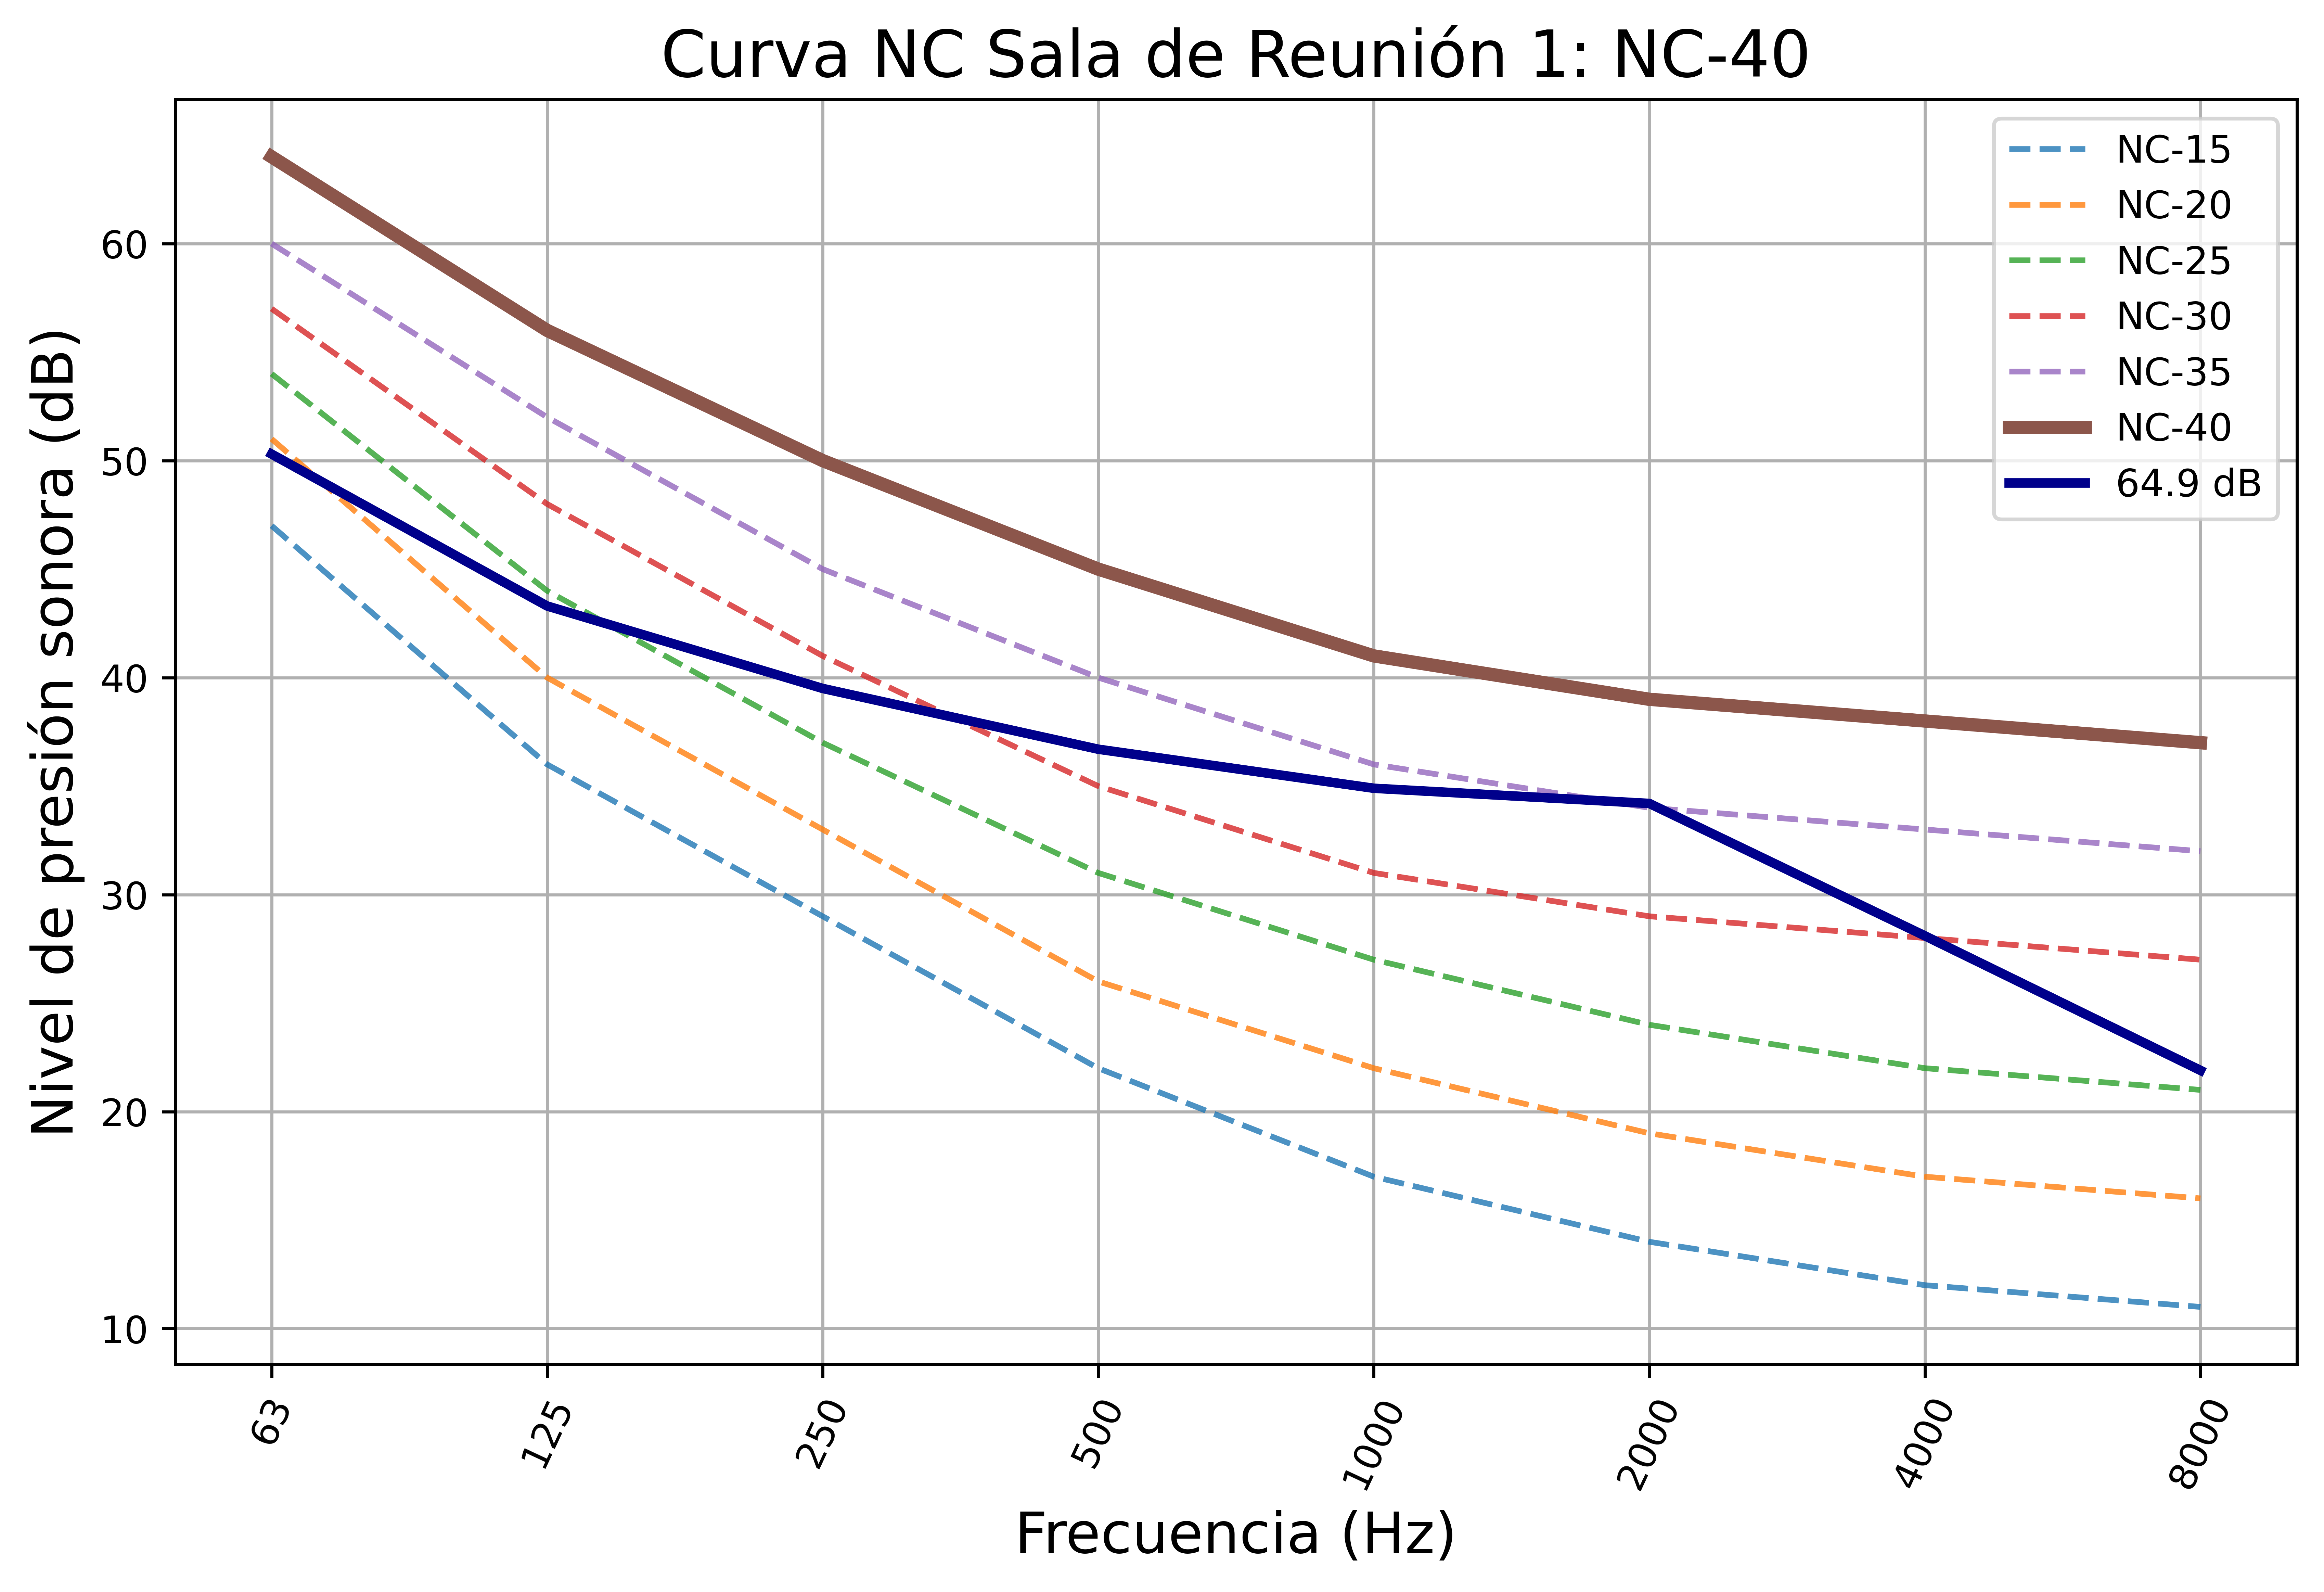
\includegraphics[width=10cm]{Imagenes/Resultados/Curvas NC-NR/NC reunion 1.png}
        \caption{Curvas NC sala de reunión 1}
        \label{fig: Curvas NC sala 1}
    \end{figure}

    \begin{figure}[H]
        \centering
        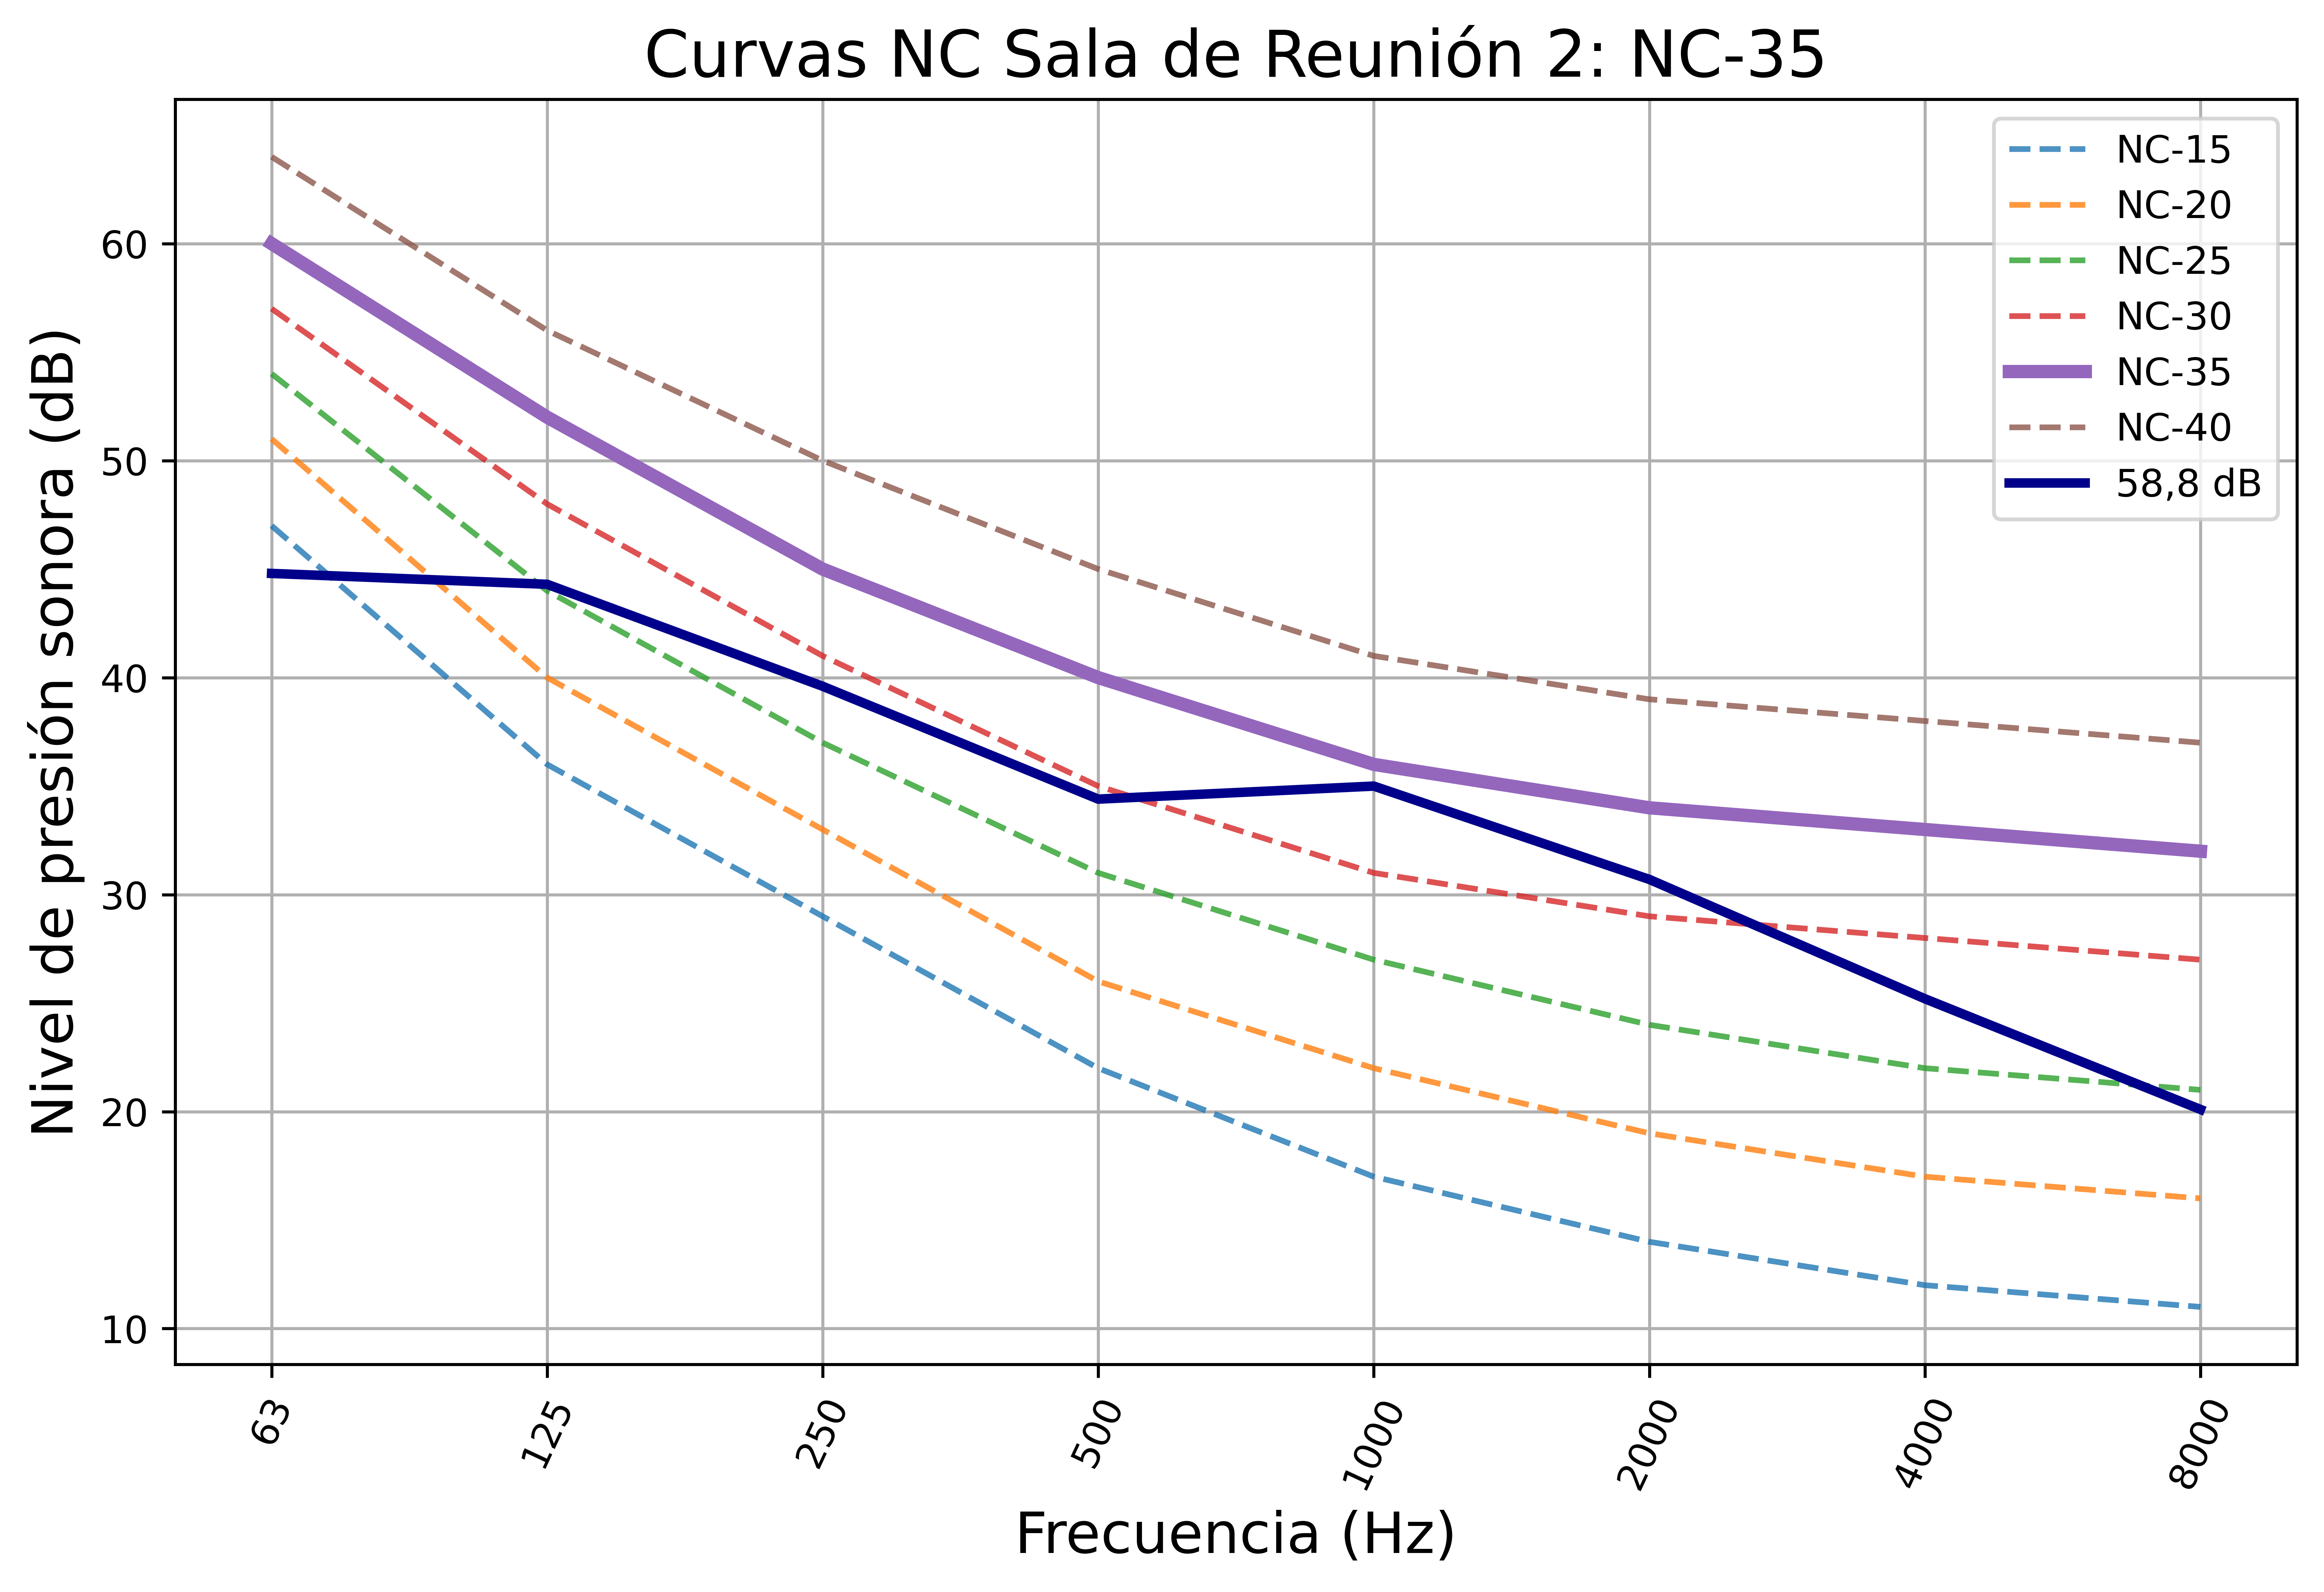
\includegraphics[width=10cm]{Imagenes/Resultados/Curvas NC-NR/NC reunion 2.png}
        \caption{Curvas NC sala de reunión 2}
        \label{fig: Curvas NC sala 2}
    \end{figure}

    \begin{figure}[H]
        \centering
        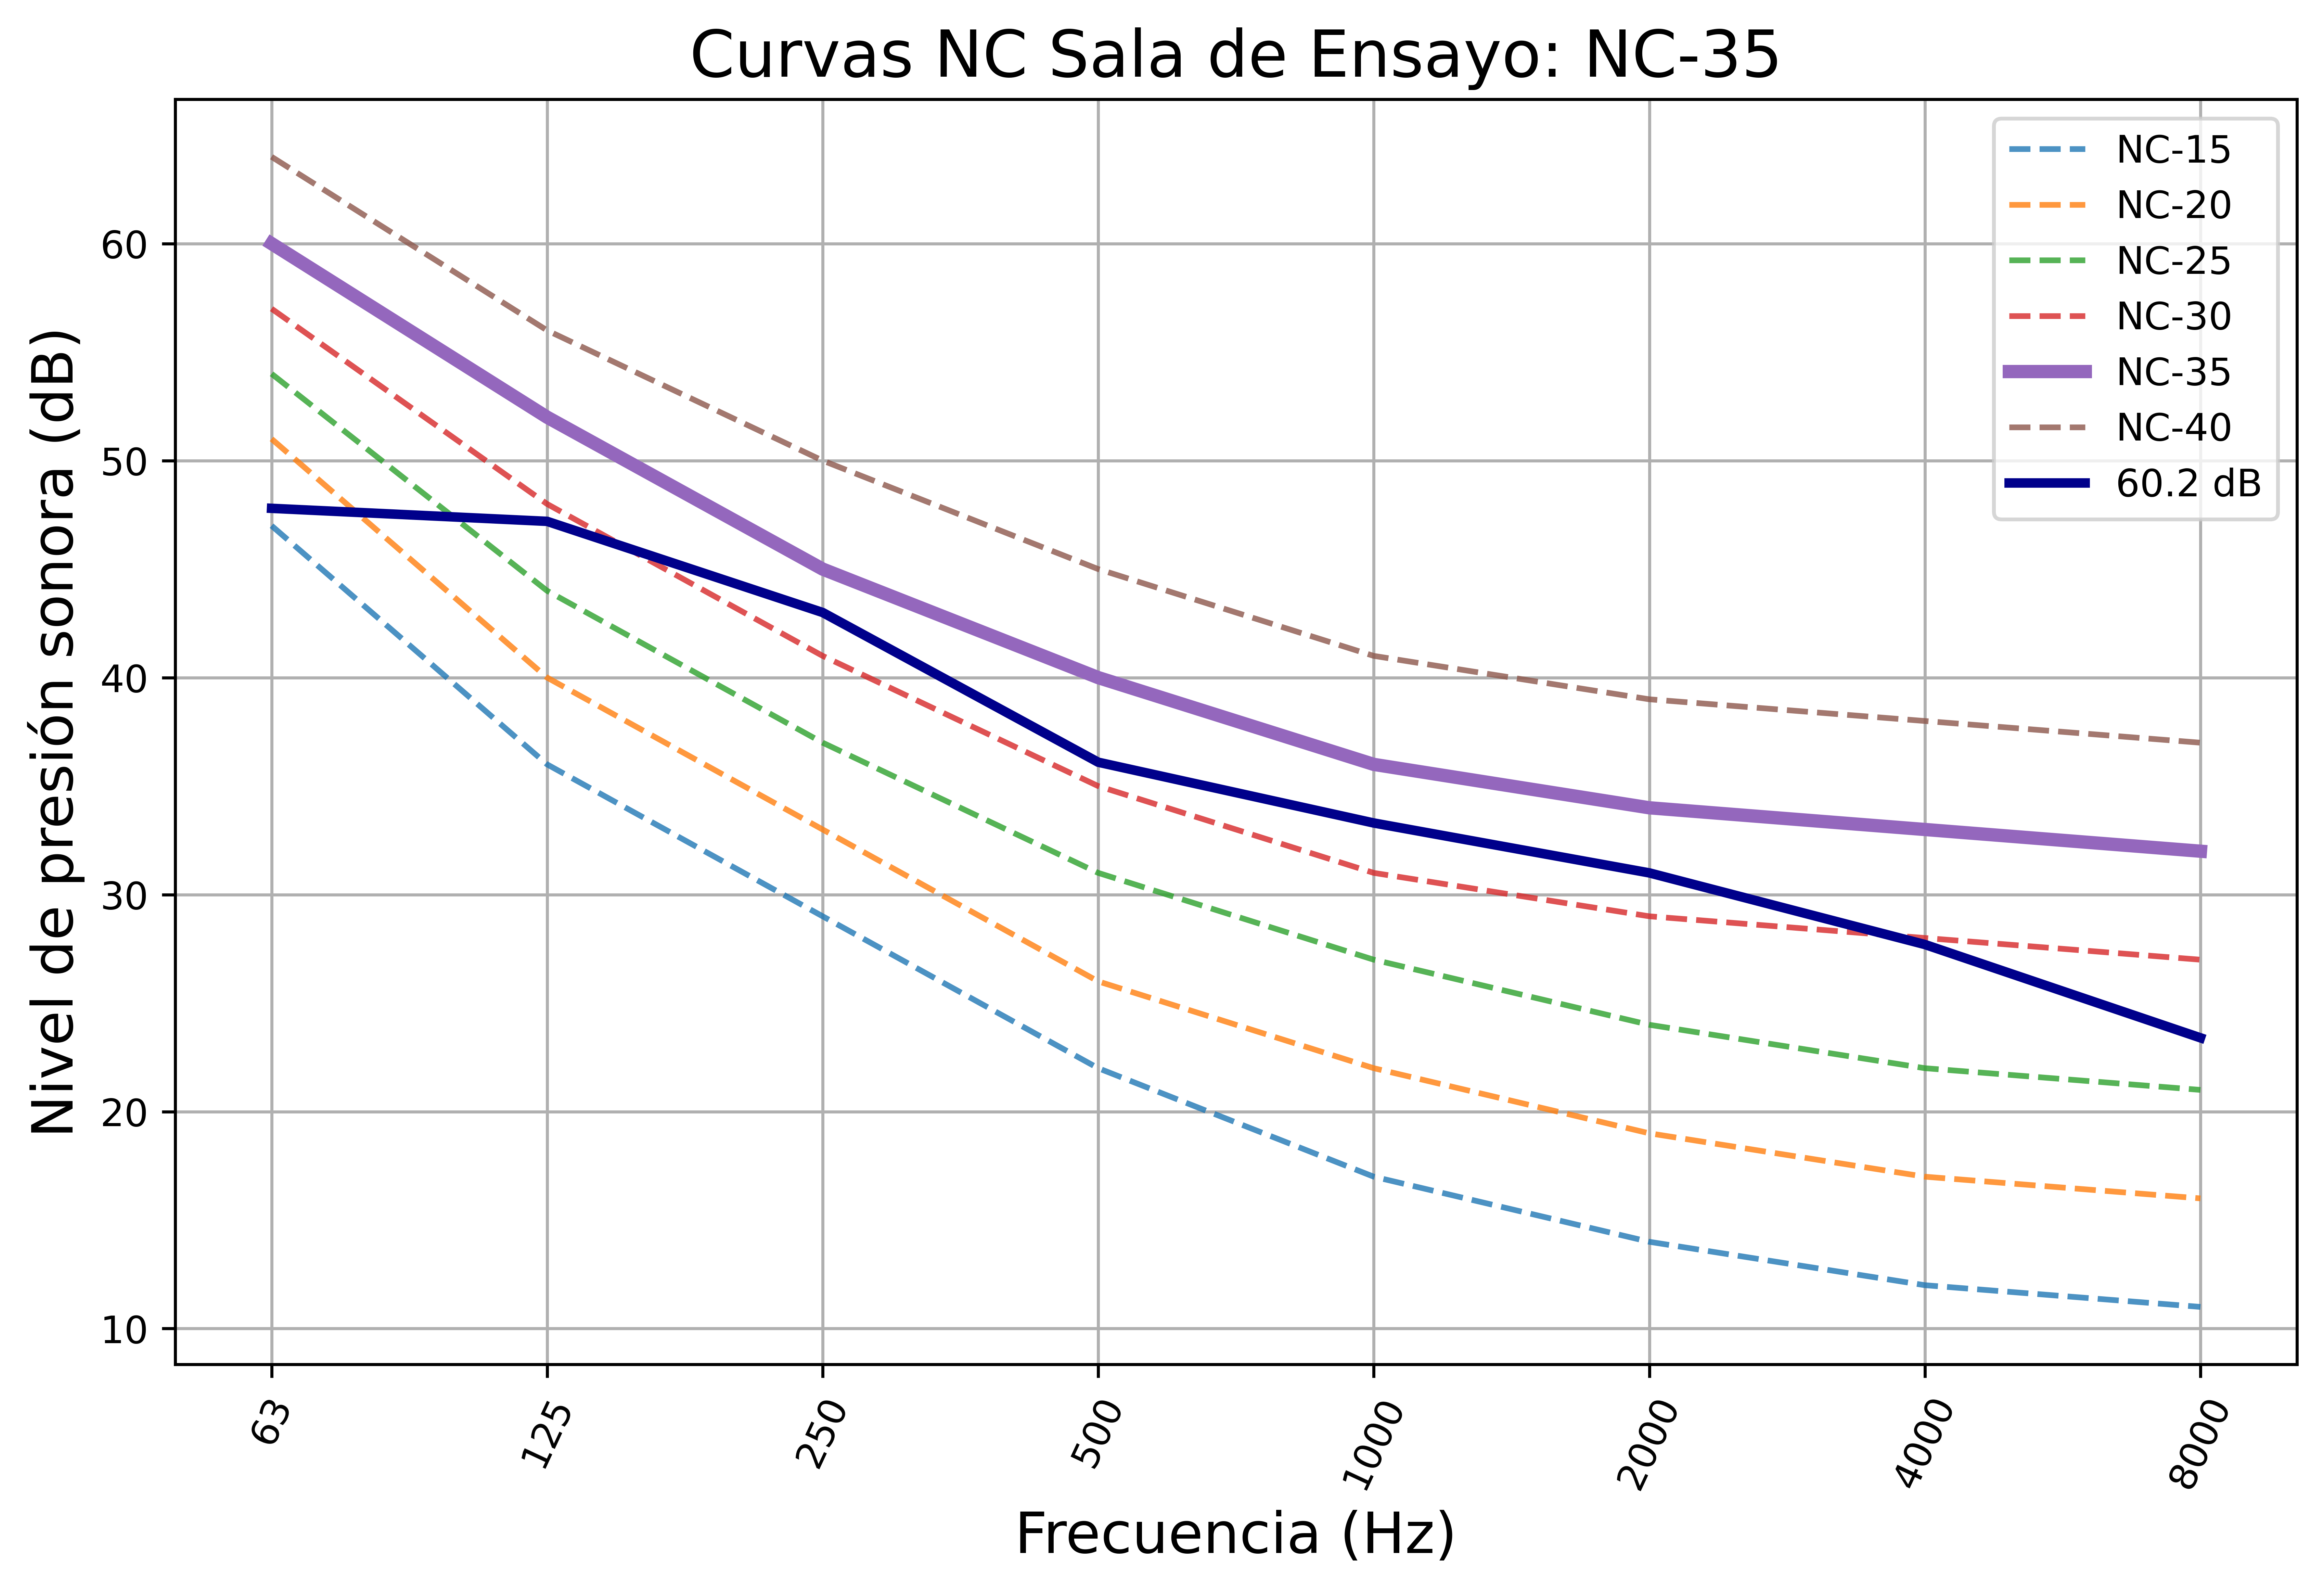
\includegraphics[width=10cm]{Imagenes/Resultados/Curvas NC-NR/NC ensayo.png}
        \caption{Curvas NC sala de ensayo}
        \label{fig: Curvas NC sala de ensayo}
    \end{figure}
    
    \item Curvas NR
    \begin{figure}[H]
        \centering
        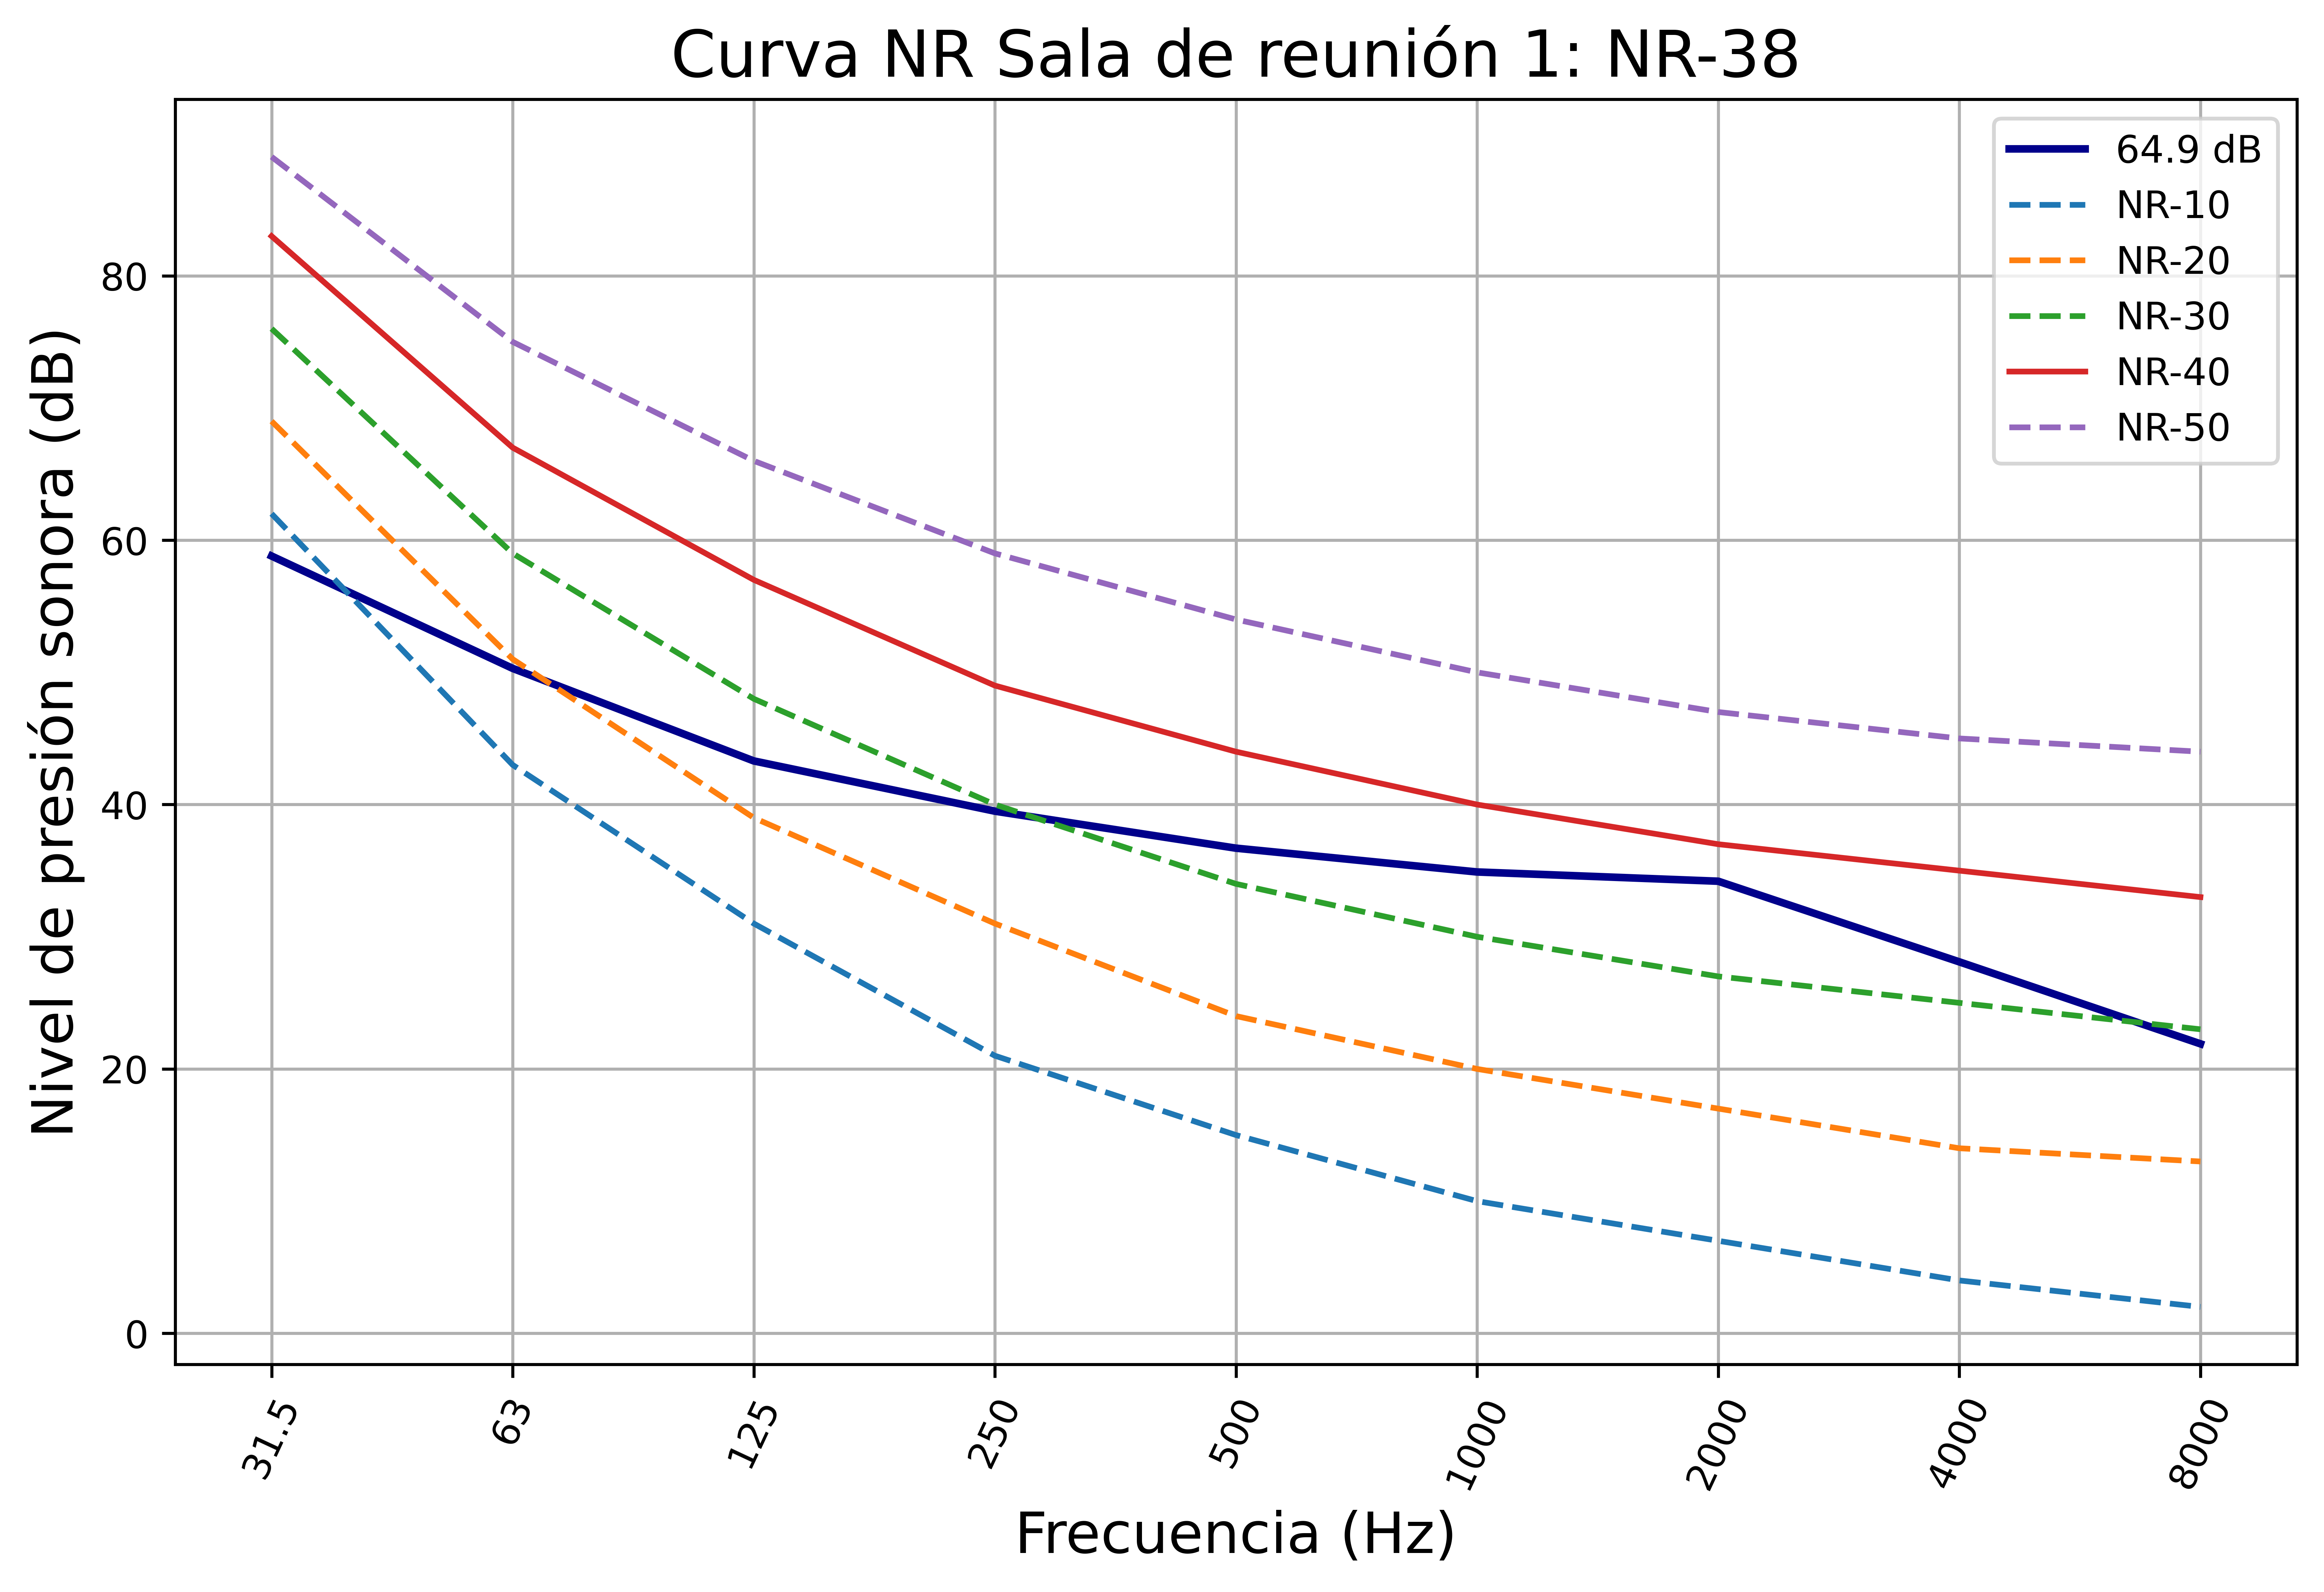
\includegraphics[width=10cm]{Imagenes/Resultados/Curvas NC-NR/NR reunion 1.png}
        \caption{Curvas NR sala de reunión 1}
        \label{fig: Curvas NR sala 1}
    \end{figure}

    \begin{figure}[H]
        \centering
        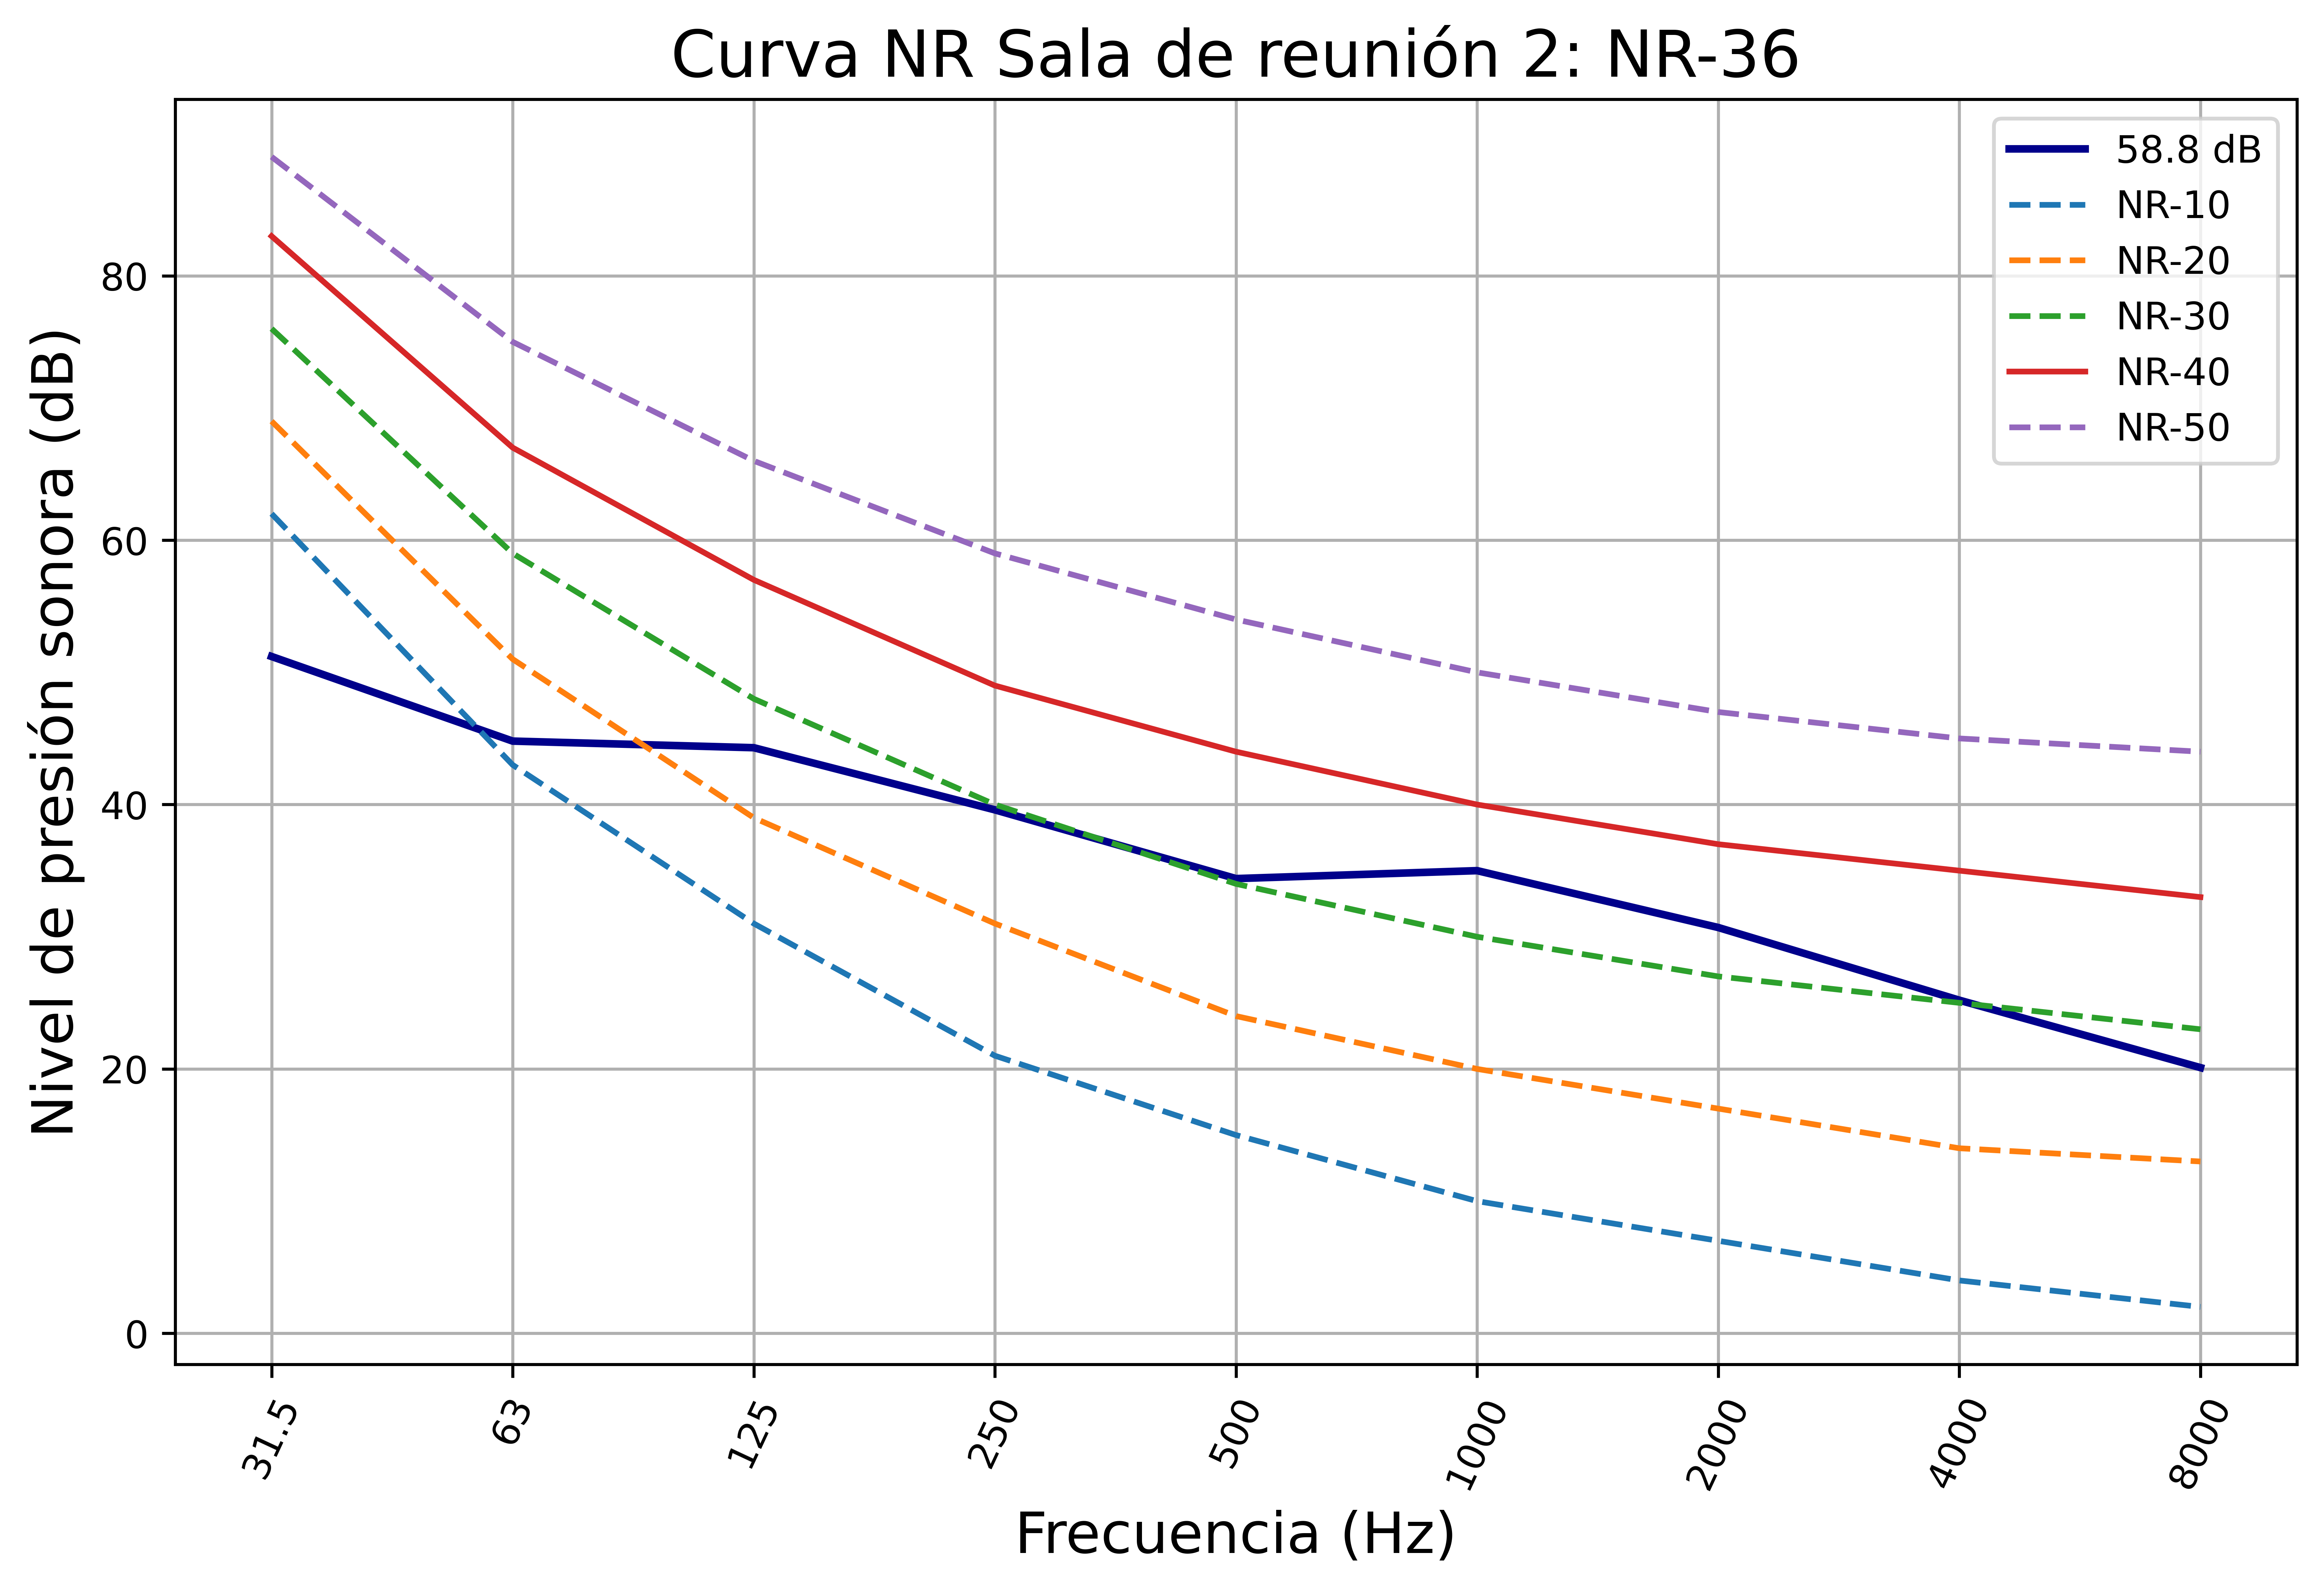
\includegraphics[width=10cm]{Imagenes/Resultados/Curvas NC-NR/NR reunion 2.png}
        \caption{Curvas NR sala de reunión 2}
        \label{fig: Curvas NR sala 2}
    \end{figure}

    \begin{figure}[H]
        \centering
        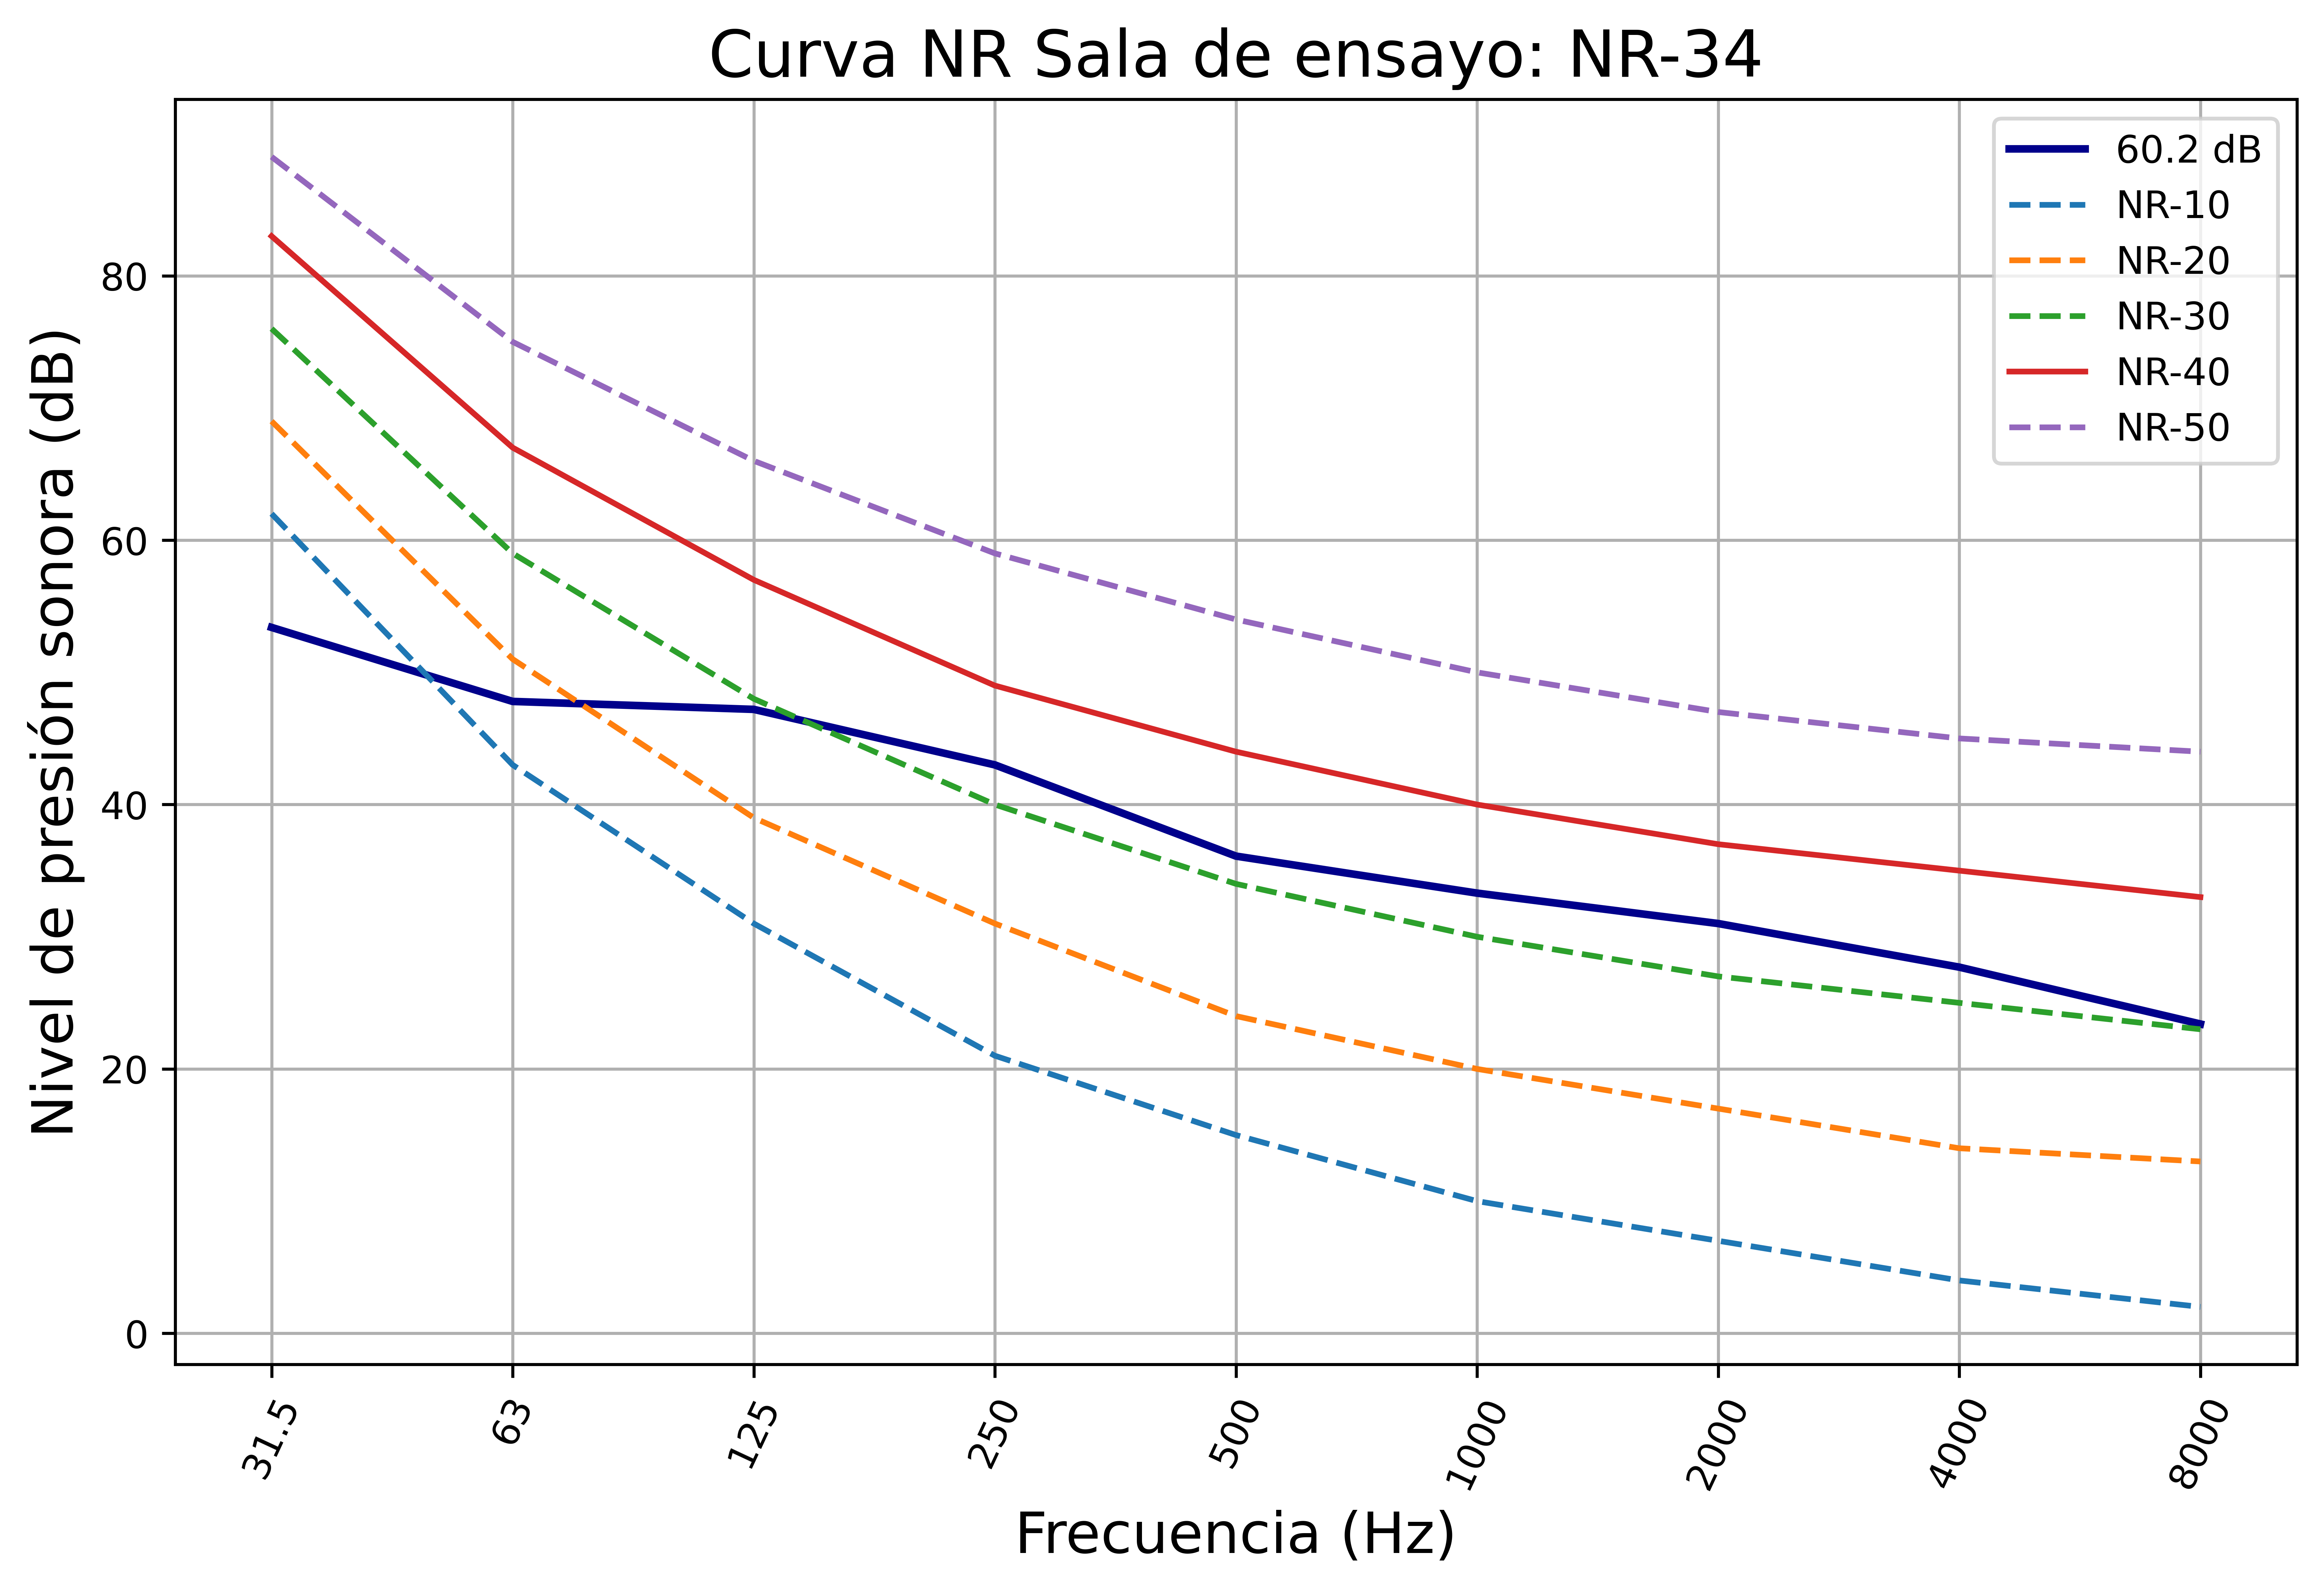
\includegraphics[width=10cm]{Imagenes/Resultados/Curvas NC-NR/NR ensayo.png}
        \caption{Curvas NR sala de ensayo}
        \label{fig: Curvas NR sala de ensayo}
    \end{figure}
\end{itemize}
Según las recomendaciones mencionadas en la sección \ref{secc: Recomendaciones} se puede determinar que los valores de ruido de fondo como se muestran en la tabla \ref{tab: cumplimiento de Rdf} no cumplen para todas las salas.

\begin{table}[H]
    \centering
    \begin{tabular}{|l|c|l|c|l|}
    \hline
    \textbf{Salones} & \textbf{Curvas NC} & \textbf{Estado} & \textbf{Curvas NR}  & \textbf{Estado} \\ \hline
     Sala de reunión $1$ & $40$ & No cumple & $38$ & No cumple \\ \hline
     Sala reunión $2$ & $35$ & No cumple & $36$ & No cumple \\ \hline
     Sala de ensayo & $35$ & No cumple & $34$ & No cumple\\ \hline
    \end{tabular}
    \caption{Estado de parámetros de ruido de fondo por sala}
    \label{tab: cumplimiento de Rdf}
\end{table}

\subsubsection{Tiempo de reverberación}
\begin{itemize}
    \item $T_{60}$
    \begin{figure}[H]
        \centering
        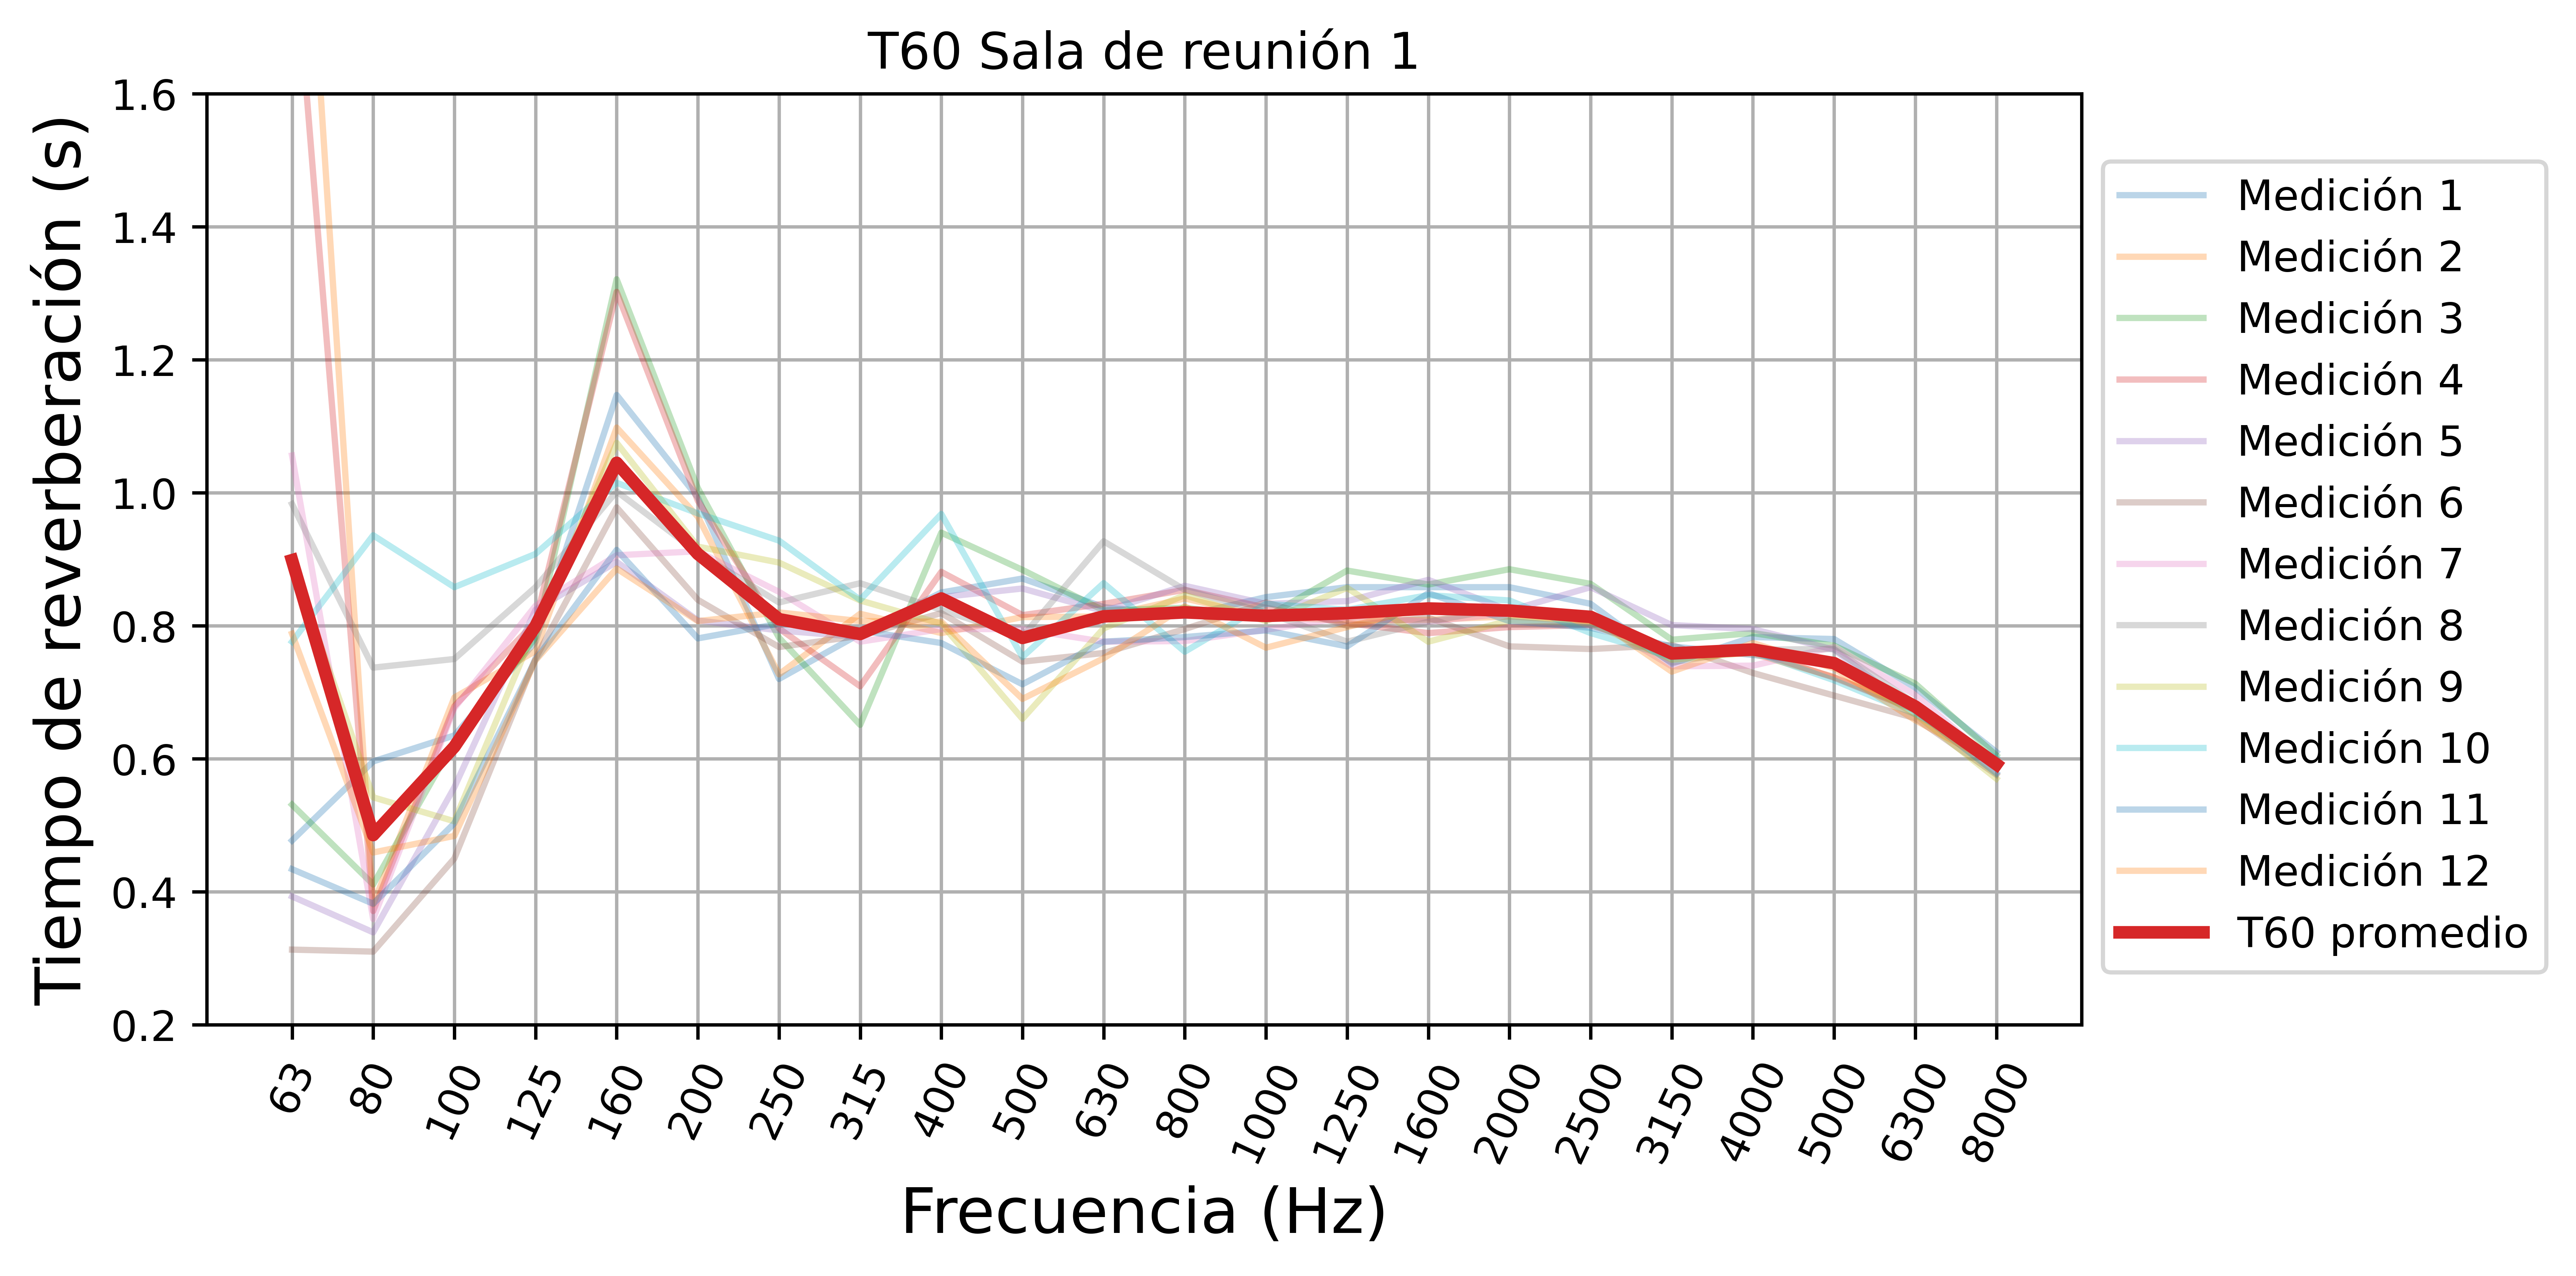
\includegraphics[width=12cm]{Imagenes/Resultados/T60_Sala_reunion_1.png}
        \caption{$T_{60}$ sala de reunión 1}
        \label{fig: T60 sala1}
    \end{figure}

    \begin{figure}[H]
        \centering
        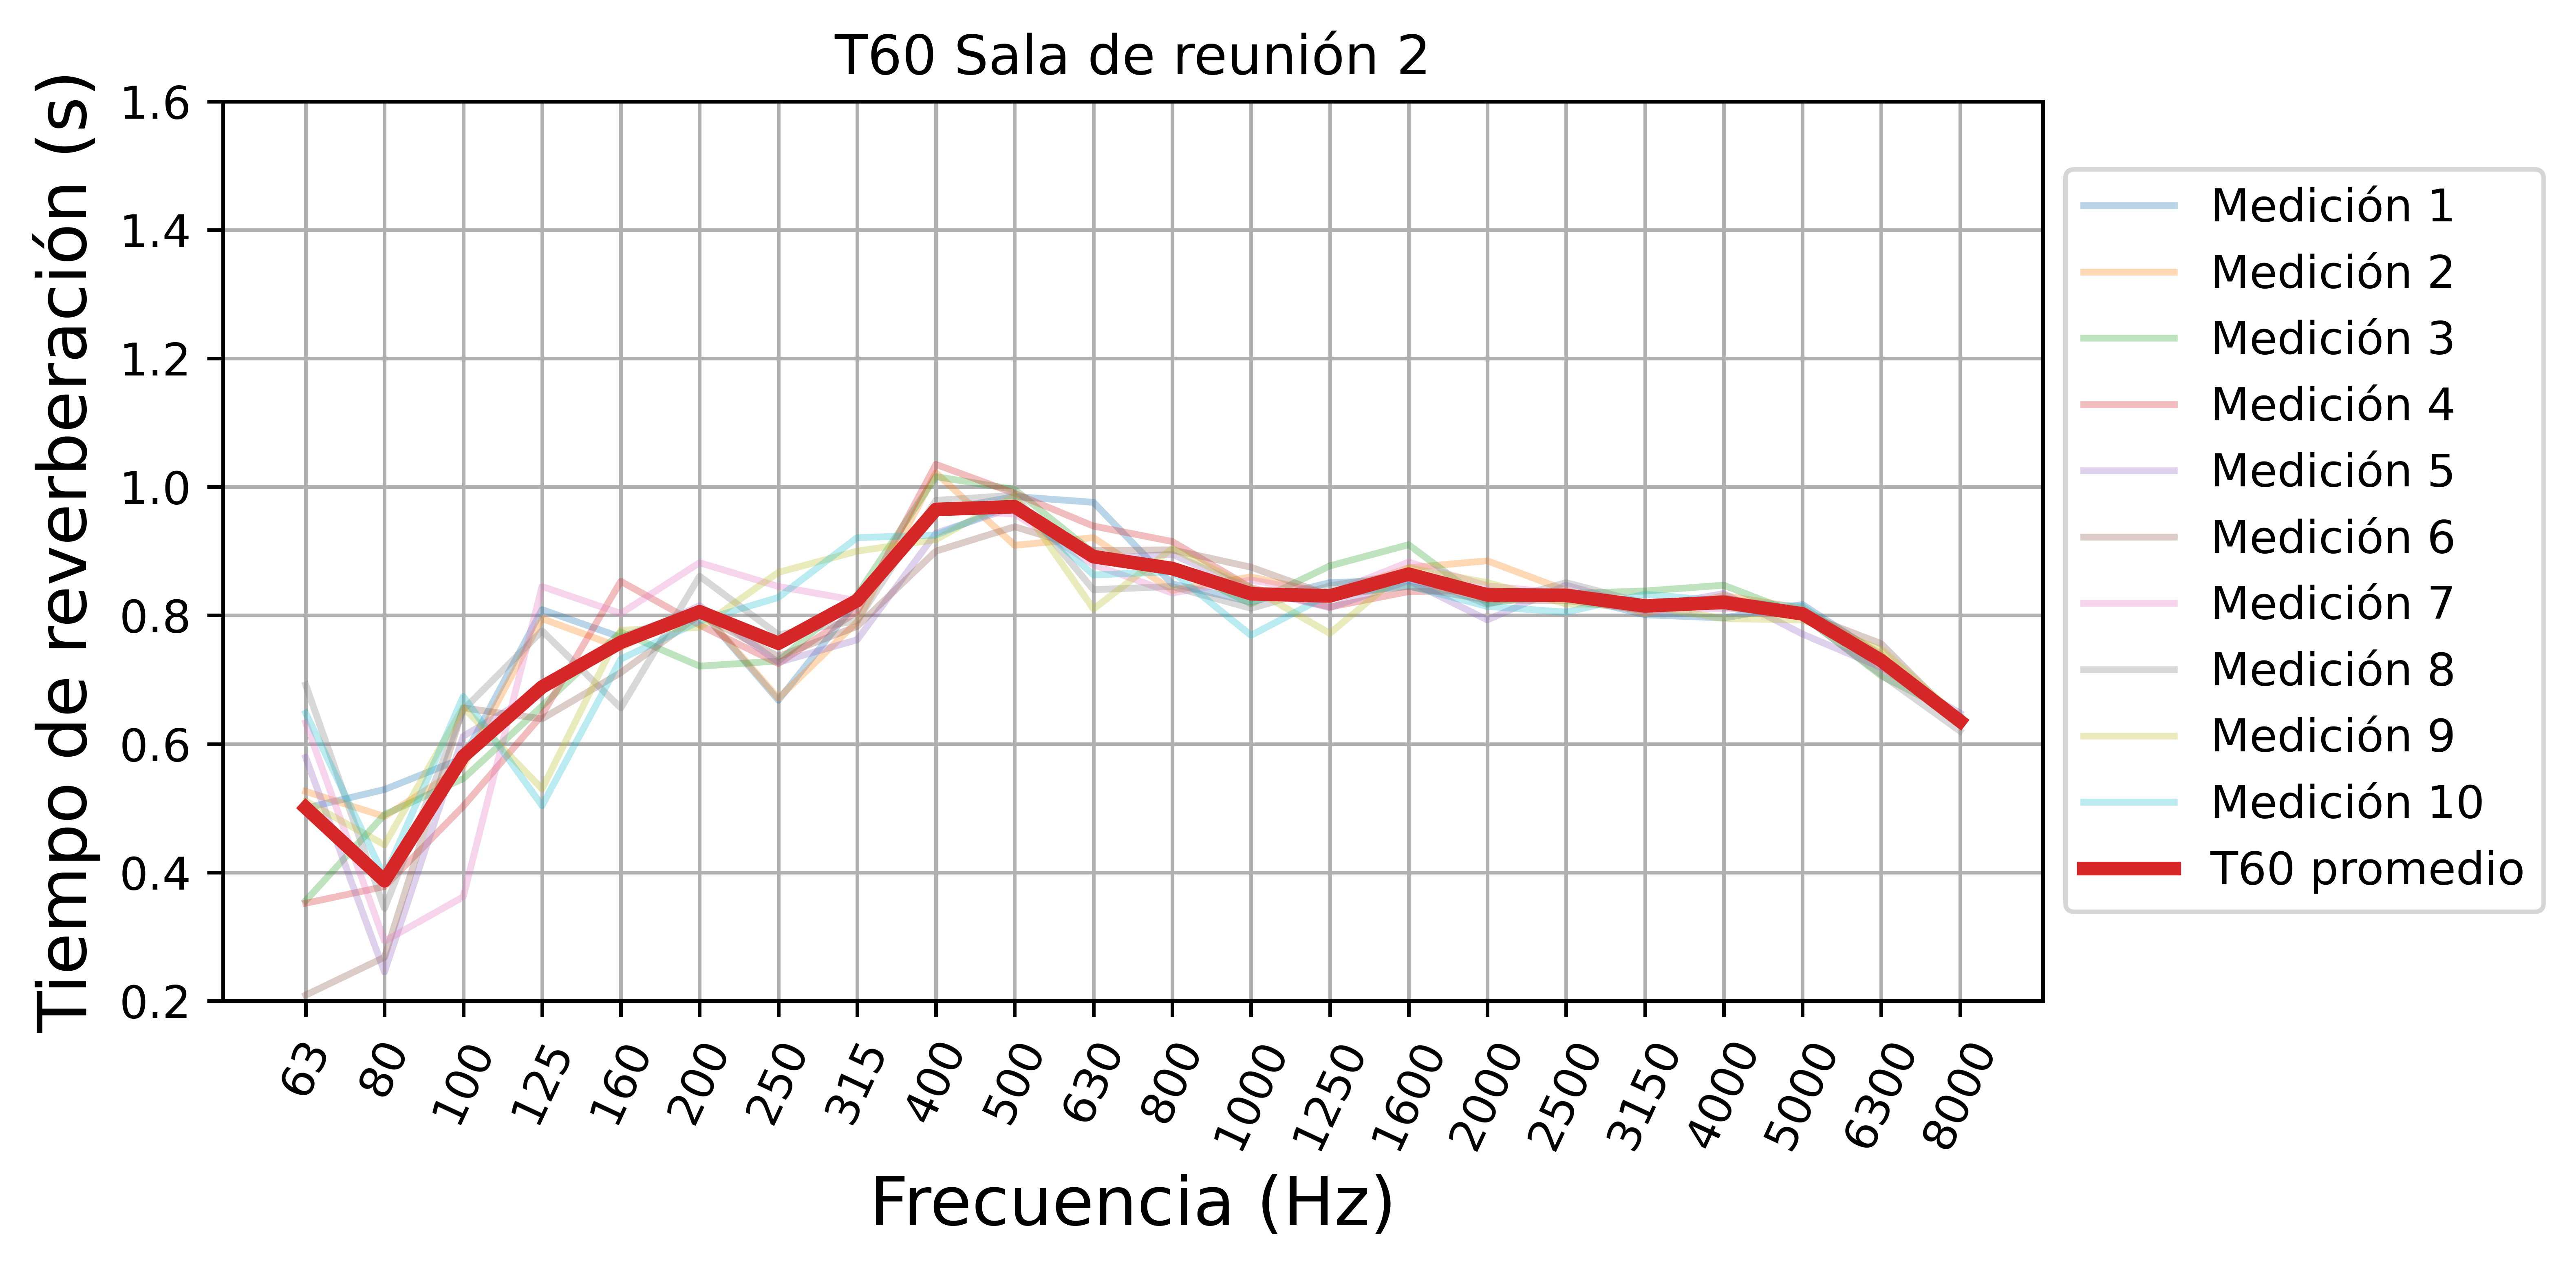
\includegraphics[width=12cm]{Imagenes/Resultados/T60_Sala_reunion_2.png}
        \caption{$T_{60}$ sala de reunión 2}
        \label{fig: T60 sala2}
    \end{figure}

    \begin{figure}[H]
        \centering
        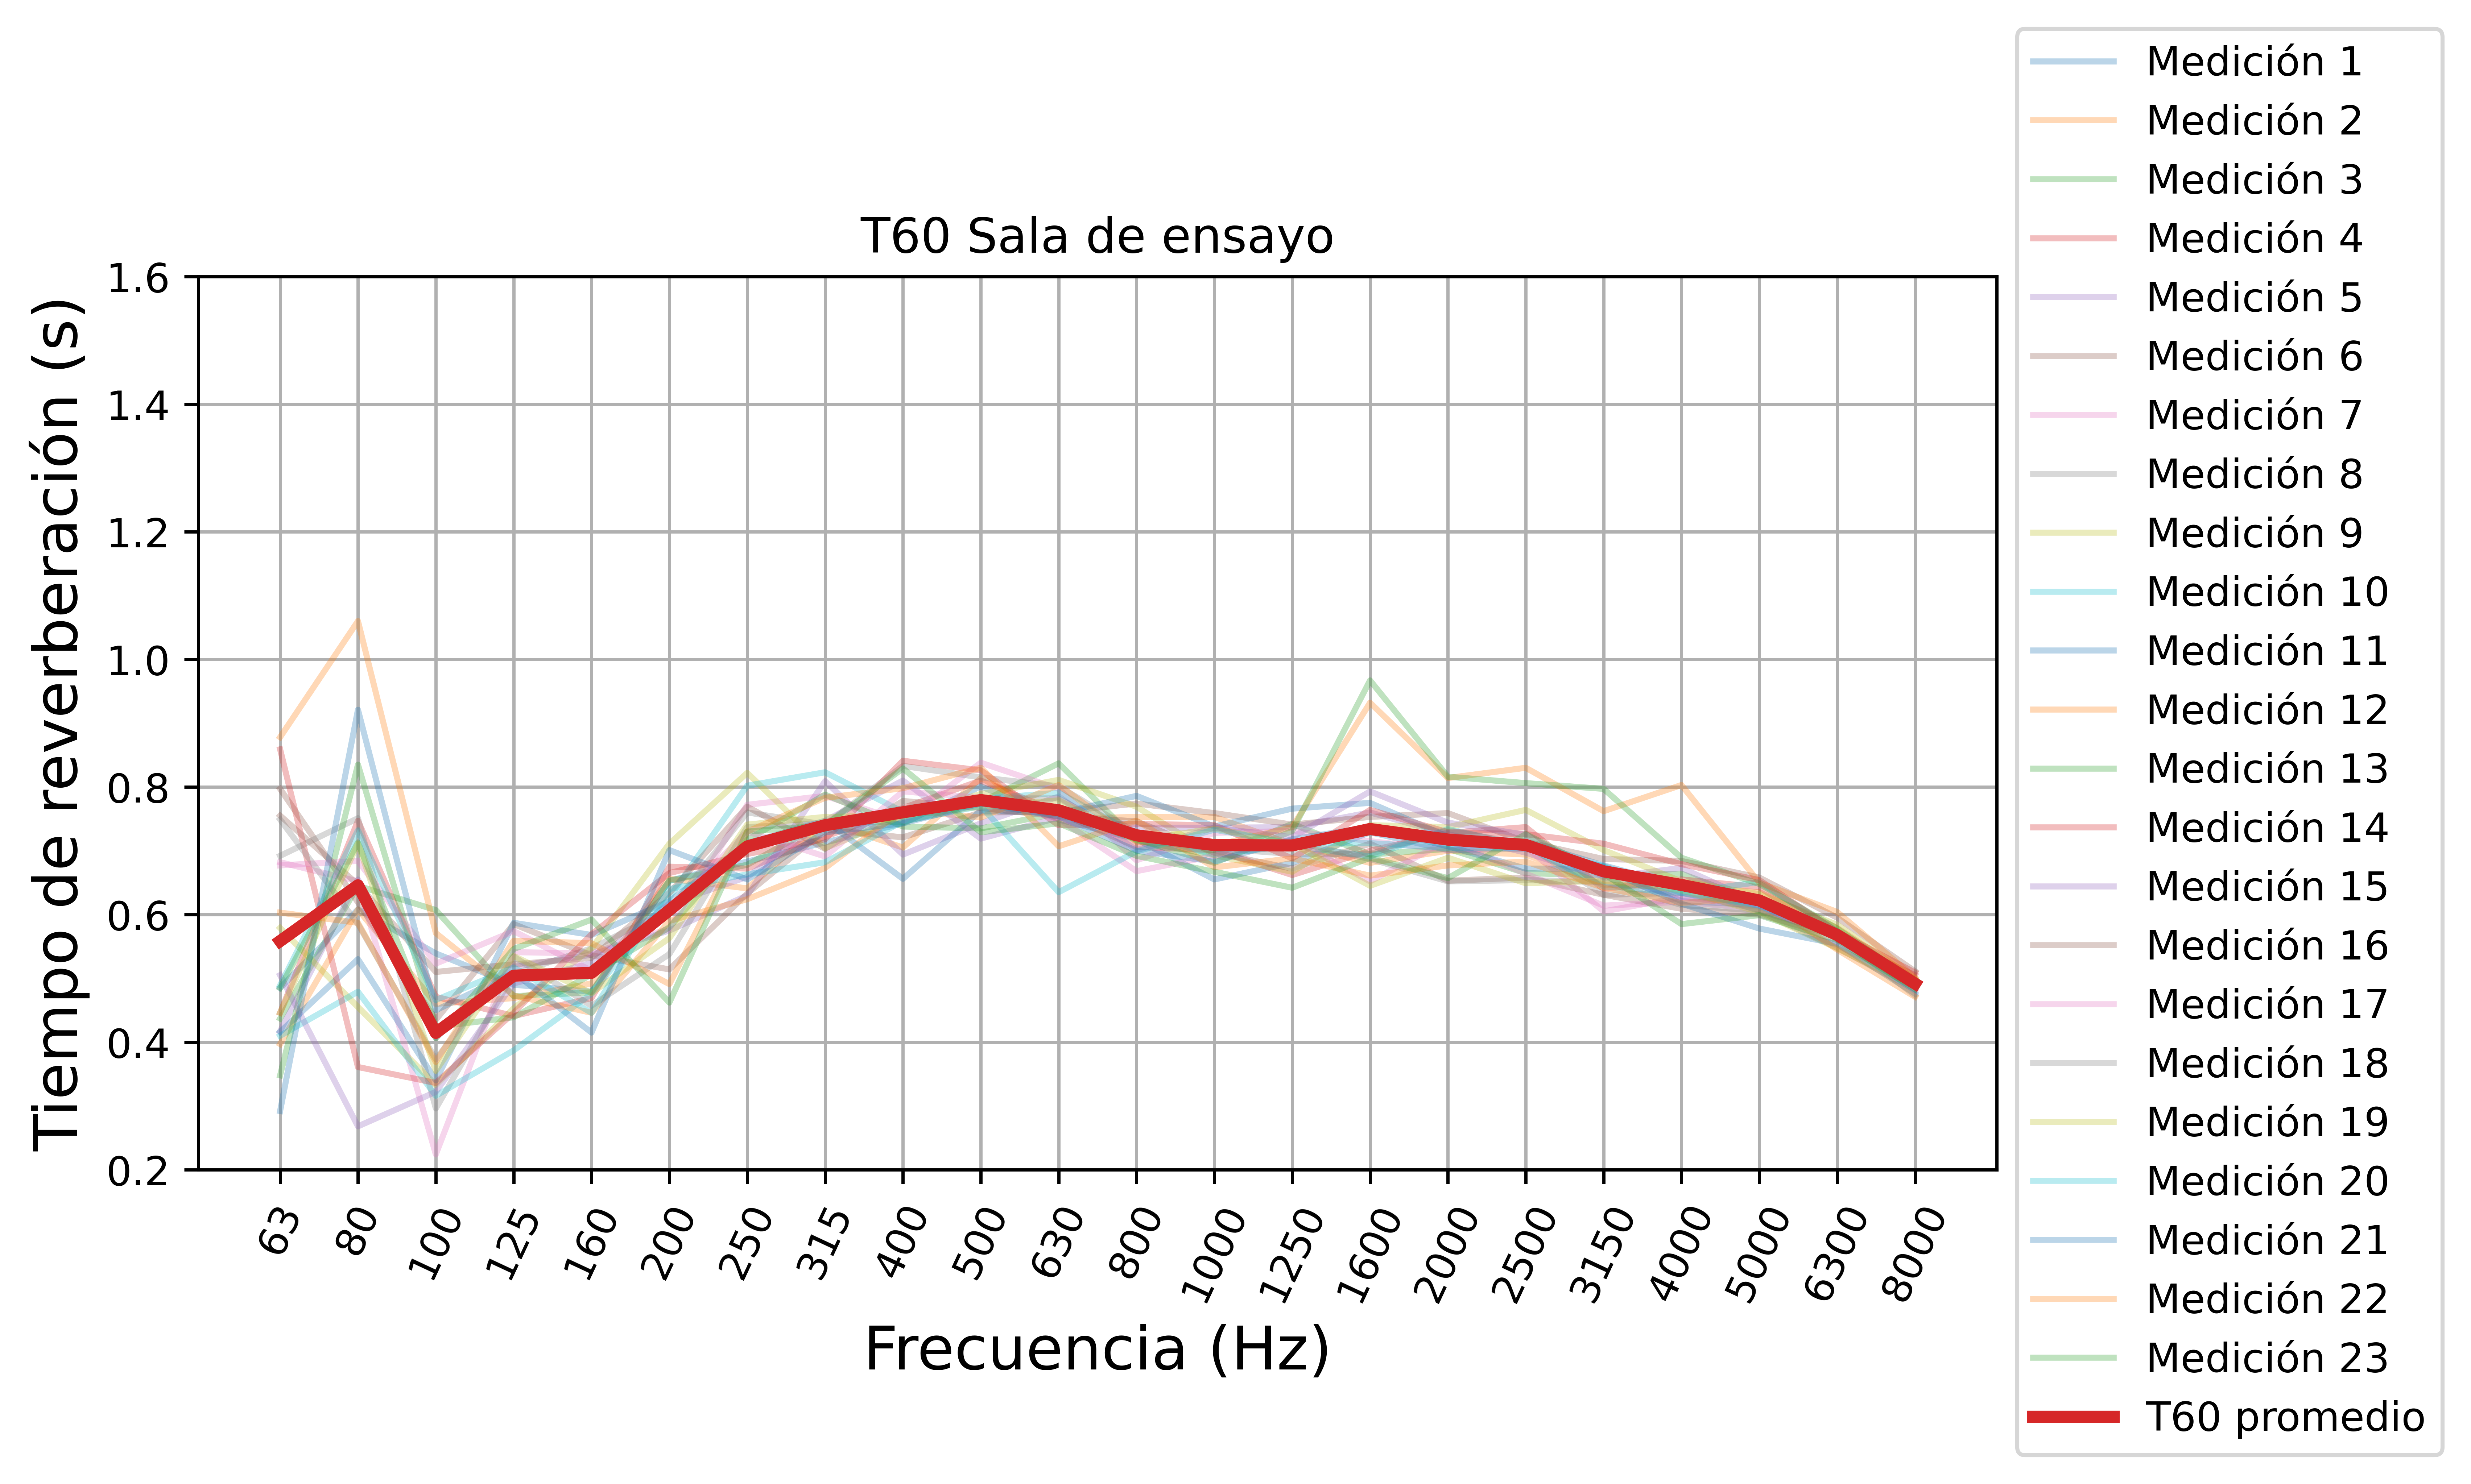
\includegraphics[width=12cm]{Imagenes/Resultados/T60_Sala_de_ensayo.png}
        \caption{$T_{60}$ sala de ensayo}
        \label{fig: T60 sala de ensayo}
    \end{figure}
    
    \item $RT_{mid}$, $C_{50}$, $C_{80}$
    A partir de los valores obtenidos de tiempo de reverberación, se determinaron parámetros como $RT_{mid}$ y claridad, parámetros que se compararon con los recomendados en la siguiente tabla. (ver tabla \ref{tab: cumplimiento parametros RT}).
    \begin{table}[H]
        \centering
        \begin{tabular}{|l|c|c|c|c|c|c|}
        \hline
          \textbf{Salón}  & $RT_{mid} (s)$ & \textbf{Estado} & $C_{50}(dB)$ & \textbf{Estado} & $C_{80} (dB)$ & \textbf{Estado}\\ \hline
          Sala de reunión $1$   &  $0.80$ & Cumple & $1.79$ & Cumple  & - & - \\ \hline
          Sala de reunión $2$   & $0.90$ & Cumple & $0.89$ & Cumple & - & - \\ \hline
          Sala de ensayo        & $0.74$ & No cumple & - & - & $6.04$ & No cumple \\ \hline
        \end{tabular}
        \caption{Parámetros acústicos de los recintos y el estado}
        \label{tab: cumplimiento parametros RT}
    \end{table}
    \item $D_{50}$ 
    También se determinó el parámetro de definición ($D_{50}$) para la sala de ensayo (ver figura \ref{fig: D50 sala de ensayo}), el cual esta fuera de lo recomendado.
    \begin{figure}[H]
        \centering
        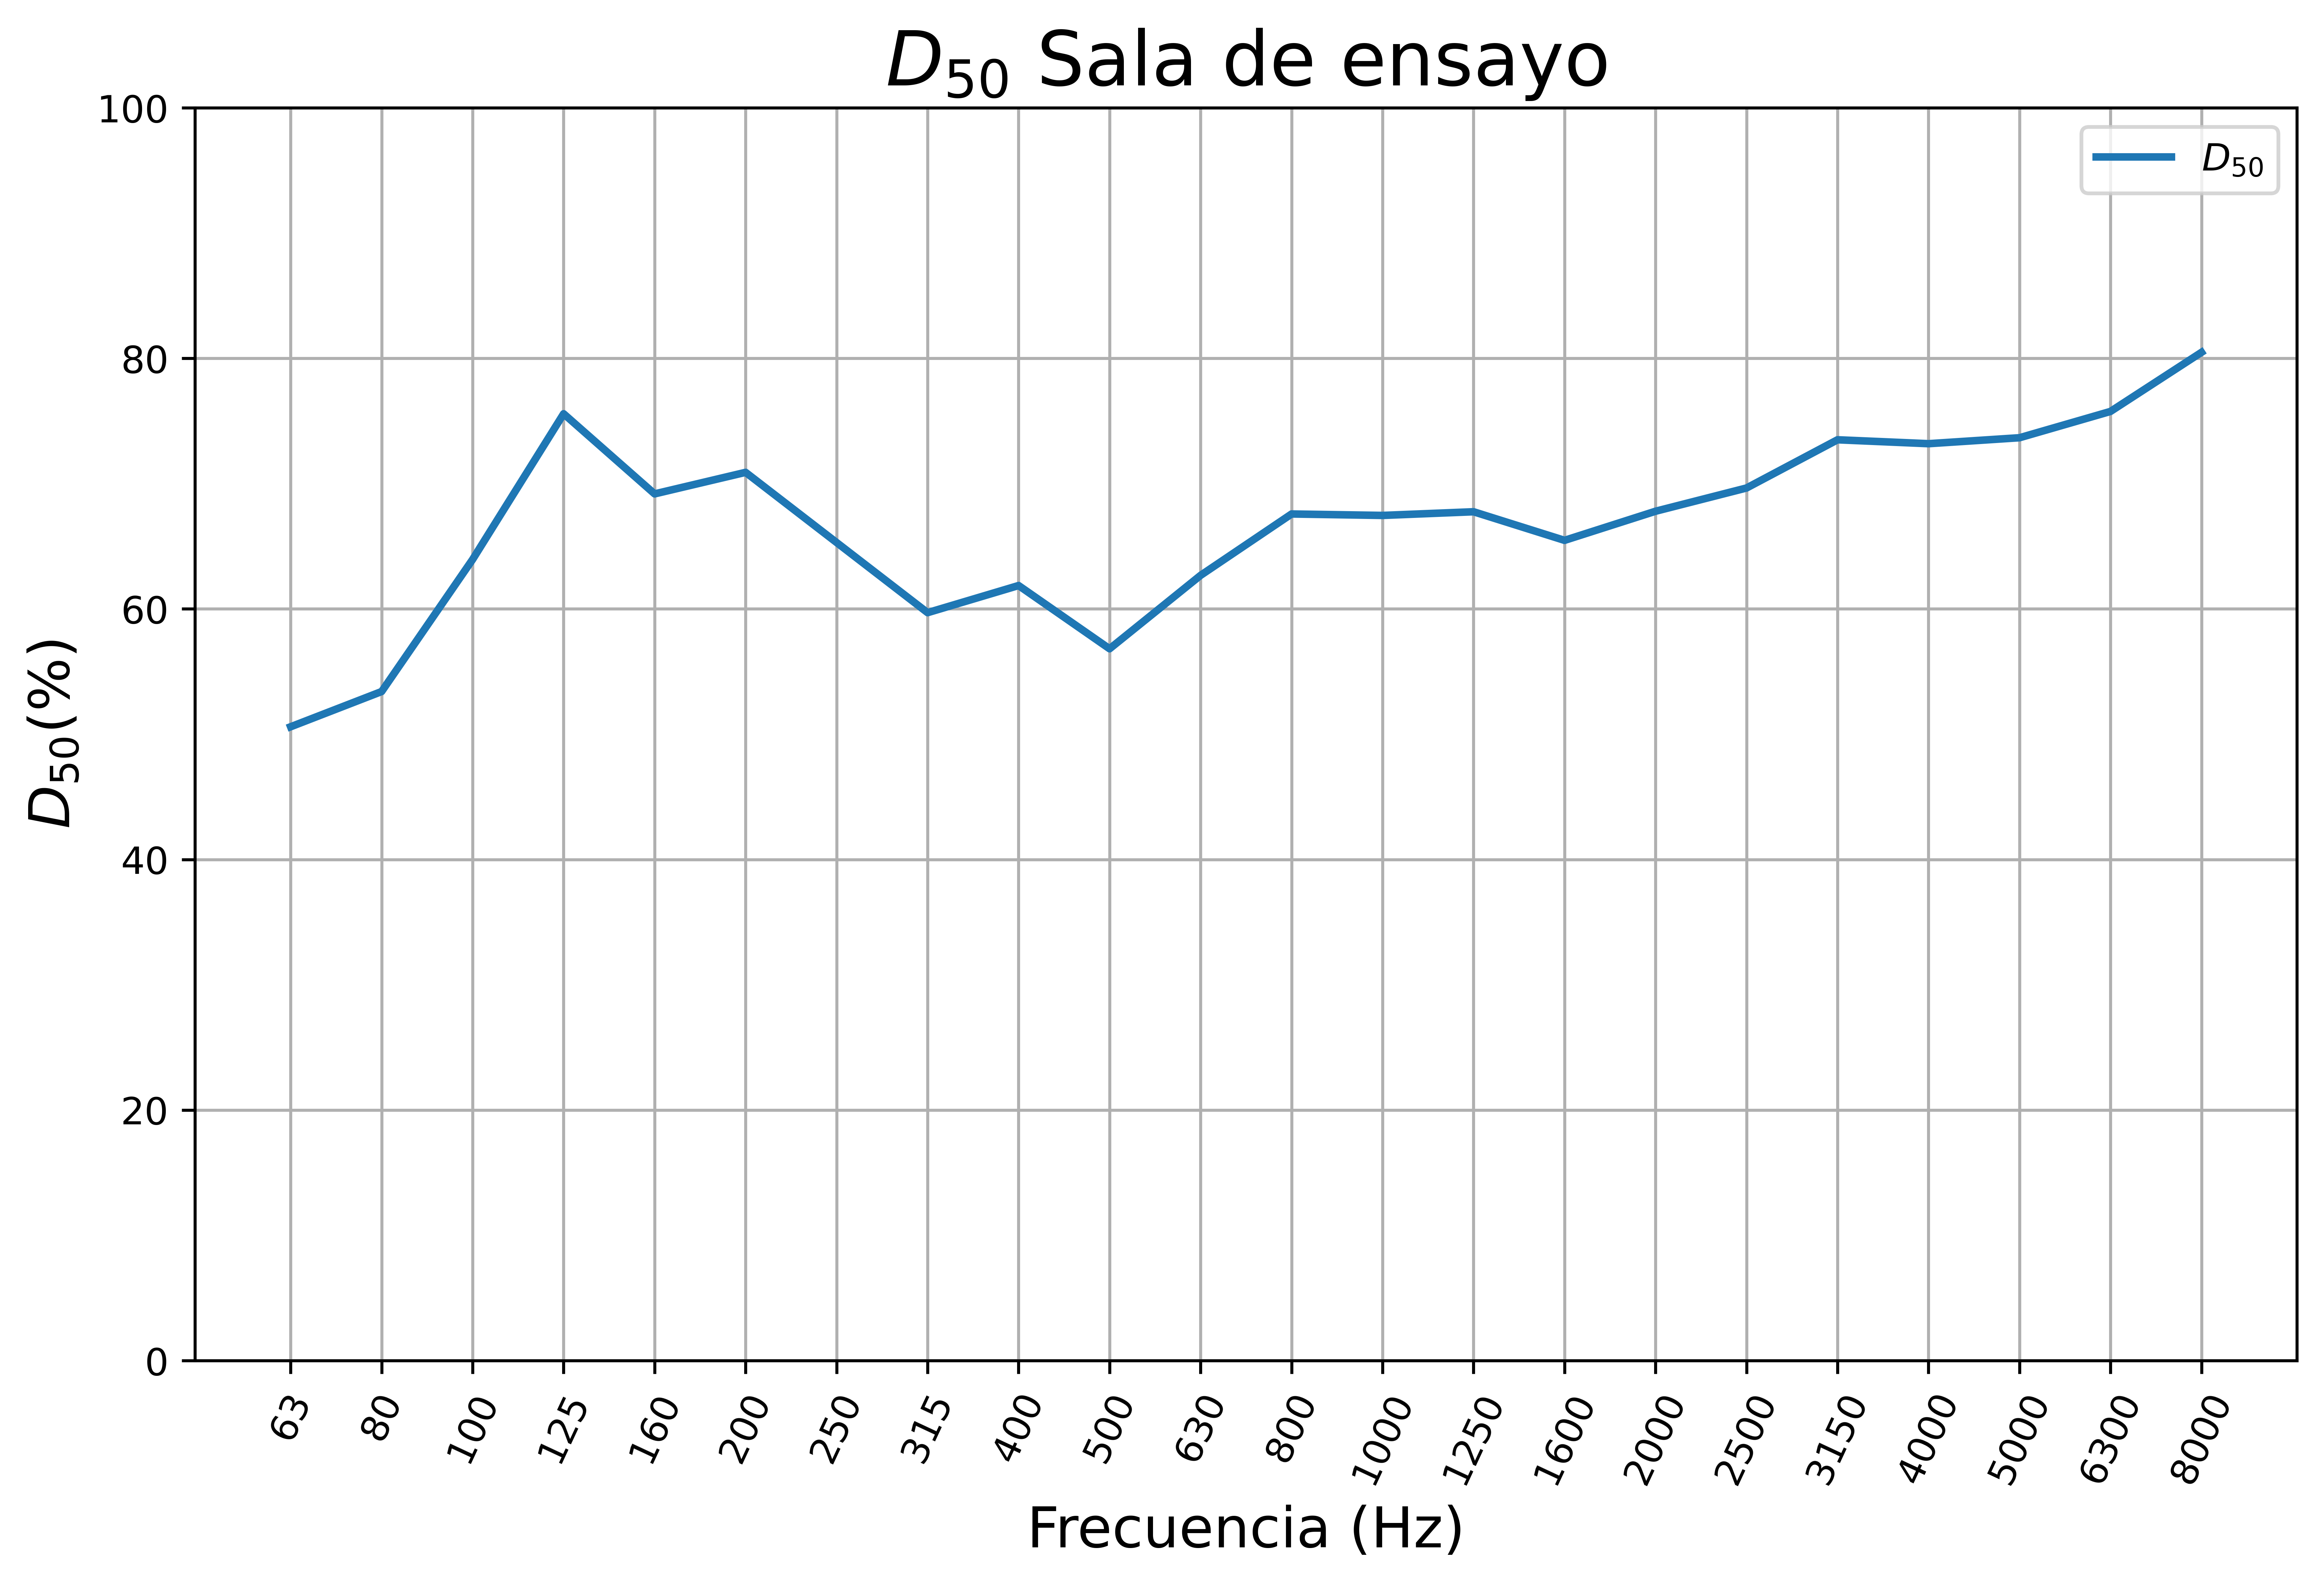
\includegraphics[scale=0.5]{Imagenes/Resultados/D50_ensayo.png}
        \caption{$D_{50}$ de sala de ensayo}
        \label{fig: D50 sala de ensayo}
    \end{figure}
\end{itemize}
